\documentclass[a4paper,11pt]{article}

\usepackage{../../zyancamlec}



\def\ntripos{Mathematical Tripos}
\def\npart{III}
\def\ncourse{Differential Geometry}
\def\nscourse{DiffGeo}
\def\nlecturer{J.\ Smith}
\def\nterm{Michaelmas}
\def\nyear{2020}

\begin{document}
	\maketitlepage
	\preliminaries

	\section*{Course Information}

	Differential geometry is the study of manifolds --- spaces built from smoothly gluing together open sets in Euclidean space —-- and structures that live on or in them. The goal of this course is to introduce the main ideas on both the abstract conceptual (‘coordinate-free’) level and the concrete computational (‘in coordinates’) level, and to develop fluency in passing between them. This will lay the foundation for future study in geometry and topology, and provide the language for modern theoretical physics. Throughout the emphasis will be on building up geometric intuition. Topics will include:


	\begin{itemize}
		\item Manifolds, tangent and cotangent spaces, smooth maps and their derivatives. Tangent and cotangent bundles, tensors. Vector fields, flows, the Lie derivative.
		\item Differential forms, the exterior derivative, de Rham cohomology. Orientability. Integration and Stokes’s theorem. Frobenius integrability.
		\item Lie groups and algebras. Principal bundles, connections (from multiple perspectives), curvature. Associated bundles, reduction of the structure group, vector bundles.
		\item Riemannian metrics, the Levi-Civita connection, geodesics and the exponential map. The Riemann tensor and its symmetries and contractions. The Hodge star, the Laplacian, statement of the Hodge decomposition.
	\end{itemize}

	
	\section*{Pre-requisites}
	
	Familiarity with point set topology (including compactness), multi-variable calculus (including the inverse function theorem), and linear algebra (including dual spaces and bilinear forms) is essential. No previous exposure to geometry will be assumed.

	\newpage
	\tableofcontents
	\newpage
	\maintext
	\section{Manifolds and Smooth Maps}
	\recnr{1}
	\subsection{Manifolds} \label{sec:1.1}
	
	A manifold is a space which locally looks like $\mathbb{R}^n$.

	\begin{defi}
		A \emph{topological $n$-manifold} is a topological space $X$ such that for every point $p$ in $X$ there exists an open neighbourhood $U$ of $p$ in $X$, an open set $V$ in $\mathbb{R}^n$, and a homeomorphism $\varphi: U \xrightarrow{\sim} V$.
		
		We also require $X$ to be 
		\begin{itemize}
			\item \emph{Hausdorff}: given distinct points $p_1$ and $p_2$ in $X$ there exist disjoint open neighbourhoods $U_1$ and $U_2$ of $p_1$ and $p_2$ respectively.
			\item \emph{second-countable}: there exists a countable collection of open sets which form a basis for the topology, i.e.\ every open set is a union of sets in the collection.
		\end{itemize}
	\end{defi}
	
	\begin{figure}[H]
		\centering
		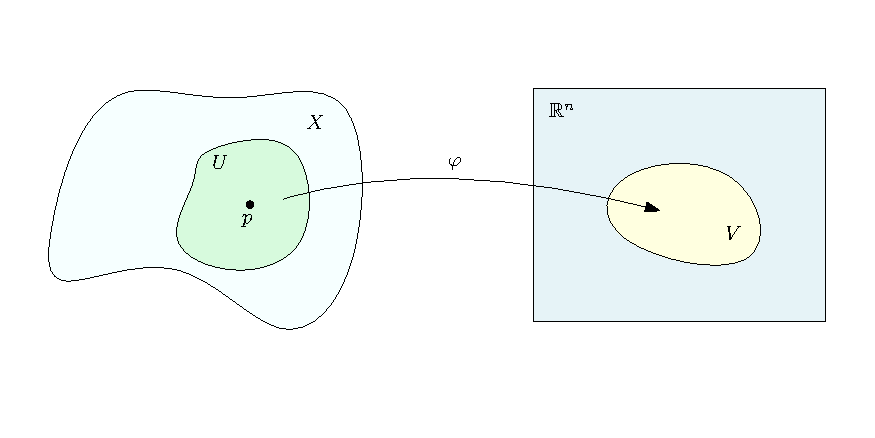
\includegraphics[width=\linewidth]{fig/fig1.pdf}
	\end{figure}

	\begin{ex}
		$\mathbb{R}^n$ is a topological $n$-manifold:
		\begin{itemize}
			\item For every $p$ take $U = V = \mathbb{R}^n$ and $\varphi = \id_{\mathbb{R}^n}$.
			\item Hausdorffness is obvious (e.g.\ since $\mathbb{R}^n$ is metrisable).
			\item A countable basis for the topology is given by open balls of rational radius with rational centre. 
		\end{itemize}
	\end{ex}

	\begin{rmk} \ 
		\begin{enumerate}
			\item Hausdorff and second-countable are important but are not restrictive in practice.
			\item They're automatic for embedded submanifolds of $\mathbb{R}^n$.
			\item They're equivalent to `$X$ is metrisable and has countably many components'.
		\end{enumerate}
	\end{rmk}

	Terminology:
	\begin{itemize}
		\item Each map $\varphi$ is a \emph{chart} (about $p$).
		\item The set $U$ is a \emph{coordinate patch}.
		\item If $x_1, \dots, x_n$ are the standard coordinates on $\mathbb{R}^n$ then
		\[
			x_1 \cpf \varphi, \dots , x_n \cpf \varphi
		\]
		are \emph{local coordinates on $U$} or \emph{local coordinates about $p$}. Usually we'll just call these $x_1, \dots , x_n$ or similar.
		\item The inverse of a chart is called a \emph{parametrisation}. (It's easier to remember which direction a parametrisation goes than a chart!)
	\end{itemize}

	\begin{ex}
		If $X$ is a topological $n$-manifold, so is any open $W \subset X$:
		\begin{itemize}
			\item If $p \in W$ and $\varphi: U \xrightarrow{\sim} V$ is a chart about $p$ in $X$ then \[
				\varphi|_{U \cap W}: W \cap W \xrightarrow{\sim} \varphi(U \cap W)
			\]
			is a chart about $p$ in $W$.
			\item Hausdorffness and second-countability are inherited from $X$.
		\end{itemize}
	\end{ex}

	More terminology:

	Given overlapping charts $\varphi: U_1 \to V_1$ and $\varphi_2 : U_2 \to V_2$, the corresponding local coordinates $x_1, \dots , x_n$ and $y_1, \dots, y_n$ are related by the \emph{transition map}
	\[
		\varphi_2 \cpf \varphi_1^{-1} : \varphi_1 (U_1 \cap U_2) \to \varphi_2 (U_1 \cap U_2).
	\]

	\begin{figure}[H]
		\centering
		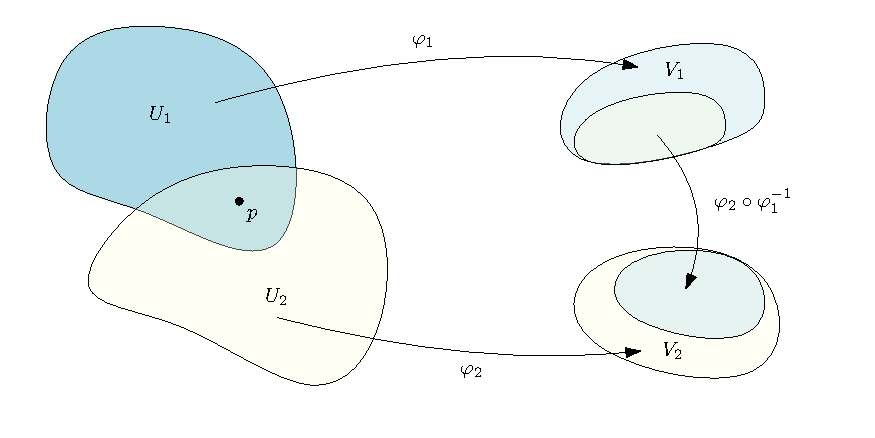
\includegraphics[width=\linewidth]{fig/fig2.pdf}
	\end{figure}
	
	This is a map between open subsets of $\mathbb{R}^n$. Such a map is \emph{smooth} if each component has all partial derivatives of all orders, i.e.\ if when we express each $y_i$ as a function of $x_1, \dots , x_n$ using $\varphi_2 \cpf \varphi_1^{-1}$ 
	\[
		\frac{\partial^k y_i}{\partial x_{j_1} \cdots \partial x_{j_k}}
	\]
	exists for all $k \geq 1$ and all $j_1, \dots , j_k$.

	We want a notion of smoothness for functions on manifolds.

	A function $f: W \to \mathbb{R}$ on an open subset $W \subset X$ may be written locally on a coordinate patch as a function $f(x_1,\dots,x_n)$ of the local coordinates.
	{\large \scshape Preliminary Definition.}\ \ $f$ is \emph{smooth} if and only if this local expression has all partial derivatives of all orders.
	{\large \scshape Problem.}\ \ On overlaps between coordinate patches this depends on the choice of local coordinates.

	A natural solution is to require all transition maps to be smooth. Then smoothness in one chart implies smoothness in other charts on overlaps, by the chain rule.

	\begin{defi} \ 
		\begin{itemize}
			\item An \emph{atlas} for a topological $n$-manifold $X$ is a collection of charts \[
				\{\varphi_\alpha: U_\alpha \xrightarrow{\sim} V_\alpha\}_{\alpha\in \mathcal{A}}
			\]
			that covers $X$, i.e.\ such that $\bigcup_{\alpha} U_\alpha = X$.
			\item An atlas is \emph{smooth} if every transition map $\varphi_\beta \cpf \varphi_\alpha^{-1}$ is smooth.
			\item Given an atlas $\mathfrak{A}$ and open $W \subset X$, a function $f: W \to \mathbb{R}$ is \emph{smooth with respect to $\mathfrak{A}$} if $f \cpf \varphi_\alpha^{-1}$ is smooth for all $\alpha$, i.e.\ if all local coordinate expressions $f(x_1,\dots,x_n)$ are smooth.
		\end{itemize}
	\end{defi}

	\begin{lem}
		If $\mathfrak{A}$ is smooth then $f$ is smooth if and only if for all $p$ in $W$ there exists $U_\alpha$ containing $p$ such that $f \cpf \varphi_\alpha^{-1}$ is smooth, i.e.\ if $f(x_1,\dots,x_n)$ is smooth for \emph{some} local coordinates $x_1, \dots,x_n$ about $p$. 
	\end{lem}

	\begin{cor}
		Given a smooth atlas $\mathfrak{A}$ all local coordinate functions are smooth with respect to the atlas.
	\end{cor}

	We'll think of two smooth atlases as being the same if they have the same smooth functions.

	\begin{defi} \ 
		\begin{itemize}
			\item Two smooth atlases are \emph{smoothly equivalent} if and only if their union is smooth (this is an equivalence relation).
			\item A \emph{smooth structure} of $X$ is an equivalence class of smooth atlases under this relation.
			\item A \emph{smooth $n$-manifold} is a topological $n$-manifold equipped with a choice of smooth structure. We'll abbreviate it to `$n$-manifold' or even just `manifold'.
		\end{itemize}
	\end{defi}

	\begin{lem}
		If $\mathfrak{A}$ and $\mathfrak{B}$ are smoothly equivalent then $f: W \to \mathbb{R}$ is smooth with respect to $\mathfrak{A}$ if and only if it's smooth with respect to $\mathfrak{B}$.
	\end{lem}

	\begin{defi}
		Given a smooth $n$-manifold $X$, a function $F: W \to \mathbb{R}$ is \emph{smooth} if and only if it's smooth with respect to some (or, equivalently, all) smooth atlas(es) representing the smooth structure.
	\end{defi}

	\begin{ex}
		$\mathbb{R}^n$ is naturally an $n$-manifold via the atlas
		\[
			\{\id: \mathbb{R}^n \xrightarrow{\sim}\mathbb{R}^n\}
		\]
	\end{ex}
	\begin{ex}
		If $X$ is an $n$-manifold, then any open $W \subset X$ inherits the structure of an $n$-manifold, by restricting charts on $X$ to $W$.
	\end{ex}

	\begin{ex}
		If $X$ is an $n$-manifold and $Y$ and $m$-manifold then $X \times Y$ is naturally an $(m+n)$-manifold, by equipping it with the product topology and the smooth structure induced by products of charts on $X$ and $Y$.
	\end{ex}

	\begin{rmk} \ 
		\begin{enumerate}
			\item Being a topological $n$-manifold is a \emph{property}.
			\item Being a smooth $n$-manifold is a property (being a topological $n$-manifold and admitting a smooth structure) \emph{plus} a choice of smooth structure.
			\item When $n = 1,2,$ or $3$, every topological $n$-manifold admits an essentially unique smooth structure.
			\item For $n \geq 4$ a topological $n$-manifold may admit no smooth structure (e.g.\ the $E_8$ manifold) or many essentially different smooth structures (e.g.\ exotic 7-spheres, or exotic $\mathbb{R}^4$). But these results are hard. 
		\end{enumerate}
	\end{rmk}

	\begin{defi}
		The integer $n$ is the \emph{dimension} of $X$, denoted $\dim X$.
	\end{defi}

	\begin{rmk} \ 
		\begin{enumerate}
			\item We'll show that a (non-empty!) smooth manifold has a unique dimension.
			\item A topological manifold also has a unique dimension but this requires algebraic topology to prove. It's at least as hard as showing $\mathbb{R}^m$ and $\mathbb{R}^n$ are not homeomorphic for $m \neq n$.
			\item A manifold of negative dimension is empty.
		\end{enumerate}
	\end{rmk}

	Conventions:
	\begin{itemize}
		\item Whenever we talk about an atlas on a manifold, it will always implicitly be a representative of the smooth structure.
		\item If we construct a new chart then we'll say that it's \emph{compatible (with the smooth structure)} if it can be added to an atlas representing the smooth structure whilst preserving smoothness.
		\item If we say `take a chart satisfying...', or `we may assume our chart satisfies...', or similar, we mean that either our atlas already contains such a chart, or we may add the chart to our atlas (i.e.\ the chart is compatible). Adding charts in this way makes no real difference.
		\begin{ex}
			We may want a chart about $p$ contained in a given open neighbourhood $W$. To do this we can take an arbitrary chart $\varphi: U \xrightarrow{\sim} V$ about $p$ and then choose the chart
			\[
				\varphi|_{U\cap W} : U \cap W \xrightarrow{\sim} \varphi(U \cap W),
			\]
			adding it to the atlas first if necessary. 
		\end{ex}
		\item Likewise `take local coordinates satisfying...' or similar, means choose a chart whose associated coordinates have these properties, or add such a chart to the atlas if non exists.
		\begin{ex}
			Given a point $p$ in a manifold $X$ we may always choose local coordinates $x_1, \dots, x_n$ about $p$ in which $p$ is given by $\vb{x} = 0$: take any chart $\varphi: U \xrightarrow{\sim} V$ about $p$ and add the chart
			\[
				\varphi - \varphi(p): U \hme \{\vb{v} - \varphi(p): \vb{v}\in V\}
			\]
			 to the atlas if it's not already there.
		\end{ex}
	\end{itemize}

	Some people avoid this by working with the \emph{maximal atlas}, meaning the union of all atlases representing the smooth structure. But this obscures the fact that it's only the equivalence class that matters.

	\begin{ex}
		The \emph{$n$-sphere}, $S^n$, is the $n$-manifold whose underlying topological space is
		\[
			\{\vb{y} = (y_0, \dots, y_n) \in \mathbb{R}^{n+1}: \norm{\vb{y}}^2 = 1\}
		\]
		with the subspace topology, and whose smooth structure is defined by the following atlas. There are two charts $\varphi_{\pm}: U_{\pm} \hme \mathbb{R}^n$, where $U_\pm = S^n \backslash \{(\pm 1, 0, \dots, 0)\}$ and $\varphi_{\pm}$ is stereographic projection
		\[
			\varphi_{\pm}(y_0, \dots, y_n) = \frac{1}{1 \mp y_0}(y_1, \dots, y_n).
		\]
		The local coordinates $\vb{x}^\pm$ associated to $\varphi_\pm$ satisfy $x^\pm_i = y_i / (1 \mp y_0)$.

		\begin{figure}[H]
			\centering
			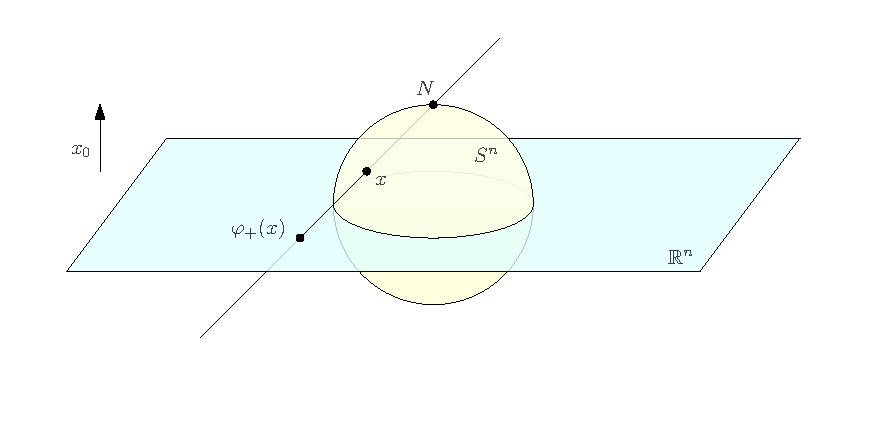
\includegraphics[width=\linewidth]{fig/fig3.pdf}
		\end{figure}

		The \emph{height function} $y_0 : S^n \to \mathbb{R}$ is smooth, since it is given by
		\[
			y_0 = \pm \frac{\norm{\vb{x}^\pm}^2 - 1}{\norm{\vb{x}^\pm}^2 + 1}\quad\text{ on }\quad U_\pm
		\]
	\end{ex}

	\begin{rmk}
		This may seem asymmetric because we singled out two points to project from, but charts obtained by stereographic projection from any other point are compatible. We'll see later that $S^n$ is a \emph{submanifold} of $\mathbb{R}^{n+1}$ and its smooth structure is inherited from $\mathbb{R}^{n+1}$. 
	\end{rmk}

	\subsection{Manifolds from Sets} \recnr{2}

	A set can be made into a manifold by identifying subsets with subsets of $\mathbb{R}^n$.

	A smooth $n$-manifold $X$ is a set equipped with:
	\begin{itemize}
		\item A topology satisfying various conditions;
		\item An (equivalence class) of smooth atlas.
	\end{itemize}

	The atlas presents $X$ as a union of sets $U_\alpha$, each identified with an open set $V_\alpha \subset \mathbb{R}^n$ by a homeomorphism $\varphi_\alpha: U_\alpha \hme V_\alpha$.

	It knows the topology on $X$: a subset $W \subset X$ is open $\Leftrightarrow$ $W \cap U_\alpha$ is open in $U_\alpha$ for all $\alpha$ $\Leftrightarrow$ $\varphi_\alpha(W\cap U_\alpha)$ is open in $V_\alpha$ for all $\alpha$.

	So we can describe $X$ by giving the underlying set, the subset $U_\alpha$, and identifications $\varphi_\alpha: U_\alpha \hme V_\alpha$ which match up smoothly.

	\begin{ex}
		We can make the set $\mathbb{C}\cup \{\infty\}$ into a manifold by covering it with $U_0 = \mathbb{C}$ and $U_\infty = \mathbb{C}^* \cup \{\infty\}$ and defining
		\begin{itemize}
			\item $\varphi_0 : U_0 \hme \mathbb{C} \cong \mathbb{R}^2$ by $\id_{\mathbb{C}}$;
			\item $\varphi_{\infty}: U_\infty \hme \mathbb{C} \cong \mathbb{R}^2$ by $z \mapsto 1/z$ on $\mathbb{C}^*$ and $\infty \mapsto 0$. 
		\end{itemize}
		The transition function $\mathbb{C}^* \to \mathbb{C}^*$ is $z \mapsto 1/z$ which is smooth.

		\begin{figure}[H]
			\centering
			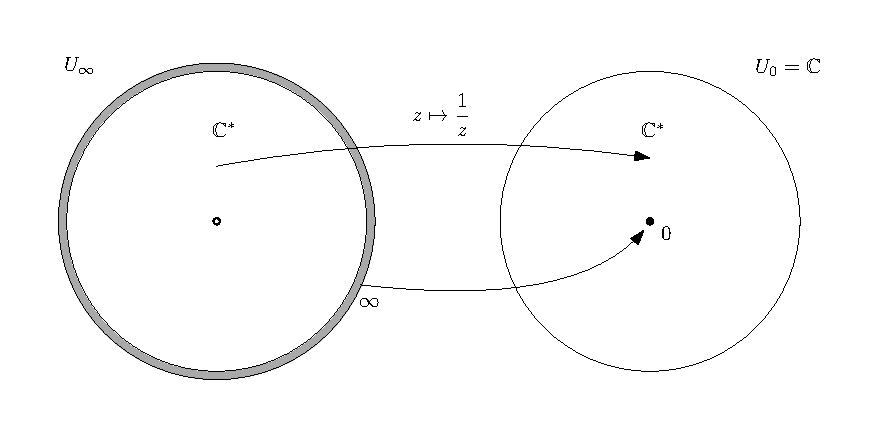
\includegraphics[width=\linewidth]{fig/fig4.pdf}
		\end{figure}

		Now check for Hausdorff property: given points $p_1 \neq p_2$, either
		\begin{itemize}
			\item They're both contained in (WLOG) $U_0$ and $\varphi_0 (p_1), \varphi_0(p_2)$ are separated by disjoint open sets in $\varphi_0 (U_0)$;
			\item Or they're $0, \infty$, separated by $\varphi_0^{-1}(\text{unit ball})$ and $\varphi_\infty^{-1}(\text{unit ball})$.
		\end{itemize}

		For second-countability: take $\varphi_0^{-1}(\text{rational balls})$ and $\varphi_\infty^{-1}(\text{rational balls})$.
	\end{ex}

	Alternative perspective:
	\begin{itemize}
		\item There's no need to talk about the underlying set;
		\item Instead we could start with open sets $V_\alpha \subset \mathbb{R}^n$ and specify how to glue them together smoothly on open subsets;
		\item The first step is then to construct the underlying set, by taking the disjoint union of the $V_\alpha$ and quotienting by the equivalence relation generated by the gluing instructions.
	\end{itemize}

	\begin{figure}[H]
		\centering
		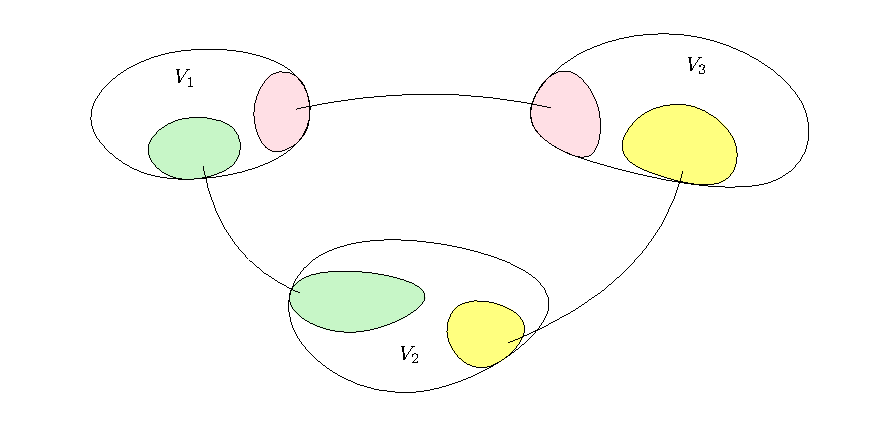
\includegraphics[width=\linewidth]{fig/fig5.pdf}
	\end{figure}

	This is `building a manifold by gluing open sets in $\mathbb{R}^n$'.

	But it's cumbersome, and one often starts with a nice description of the underlying set anyway, so we shall take it as given.

	Suppose we're given:
	\begin{itemize}
		\item A set $X$;
		\item A collection $\{U_\alpha\}_{\alpha\in \mathcal{A}}$ of subsets covering $X$;
		\item For each $\alpha$ an open set $V_\alpha \subset \mathbb{R}^n$ and a bijection $\varphi_\alpha : U_\alpha \to V_\alpha$.
	\end{itemize}
	Suppose also that for all $\alpha$ and $\beta$ in $\mathcal{A}$ the set $\varphi_\alpha(U_\alpha \cap U_\beta)$ is open in $V_\alpha$ (or, equivalently, open in $\mathbb{R}^n$), and that
	\[
		\varphi_\beta \cpf \varphi_\alpha^{-1} : \varphi_\alpha(U_\alpha \cap U_\beta) \to \varphi_\beta (U_\alpha \cap U_\beta) \subset \mathbb{R}^n
	\]
	is smooth.

	\begin{defi}
		Call the data above a \emph{smooth pseudo-atlas}, and each $\varphi_\alpha$ a \emph{pseudo-chart}. (Non-standard definition.)
	\end{defi}

	Declare a subset $W \subset X$ to be open if and only if $\varphi_\alpha(W\cap U_\alpha)$ is open in $V_\alpha$ for all $\alpha$.

	\begin{lem}
		This defines a topology on $X$.
	\end{lem}

	\begin{proof}
		Easy to check.
	\end{proof}

	\begin{prop}
		Apart from the possible failure of Hausdorff and second countable, the resulting topological space $X$ is a topological $n$-manifold and the pseudo-atlas $\{\varphi_\alpha : U_\alpha \to V_\alpha\}_{\alpha\in \mathcal{A}}$ forms a smooth atlas.
	\end{prop}

	\begin{proof}
		We just need to check that the $U_\alpha$ are open and that the pseudo-charts $\varphi_\alpha$ are homeomorphisms with respect to the topology we have defined on $X$. So take an arbitrary $\alpha$ and a subset $W \subset U_\alpha$. We need to show that $W$ is open in $X$ if and only if $\varphi_\alpha(W)$ is open in $V_\alpha$.
		
		To show $W \subset U_\alpha$ is open $\Leftrightarrow$ $\varphi_\alpha(W)$ is open in $V_\alpha$.

		$\Rightarrow$: Clear.

		$\Leftarrow$: Suppose $\varphi_\alpha(W)$ is open. Required to prove that for all $\beta$ the set $\varphi_\beta (W\cap U_\beta)$ is open in $V_\beta$. For all $\beta$ we have
		\begin{align*}
			\varphi_\beta (W \cap U_\beta) & = \varphi_\beta \cpf \varphi_\alpha^{-1} ( \varphi_\alpha (W\cap U_\beta))\\
			& = (\varphi_\alpha \cpf \varphi_\beta^{-1})^{-1} (\varphi_\alpha(W)\cap \varphi_\alpha(U_\alpha \cap U_\beta)).
		\end{align*}

		We're assuming $\varphi_\alpha(W)$ is open in $V_\alpha$ and our hypotheses mean
		\begin{itemize}
			\item $\varphi_\alpha(U_\alpha\cap U_\beta)$ is also open;
			\item $\varphi_\alpha \cpf \varphi_\beta^{-1}$ is smooth and hence continuous.
		\end{itemize}

		Thus $\varphi_\beta(W \cap U_\beta)$ is indeed open.
	\end{proof}

	Say two smooth pseudo-atlases are equivalent if their union is also a smooth pseudo-atlas.

	\begin{lem}
		Equivalent smooth pseudo-atlases define the same topology and smooth structure on $X$.
	\end{lem}

	\begin{proof}[Sketch Proof]
		Reduce to the case where one pseudo-atlas contains the other. Then check by hand.
	\end{proof}

	There's no easy general method for checking whether the topology induced by a pseudo-atlas is Hausdorff. One sufficient condition is that for all $p_1,p_2$ in $X$ some pseudo-chart $U_\alpha$ covers both points.
	
	Second-countability is much easier: it's enough for $X$ to be covered by countably many of the pseudo-charts.

	\subsection{Projective Spaces and Grassmannians} \recnr{3}

	Projective spaces and Grassmannians, parametrising subspaces of a fixed vector space are all manifolds.

	\begin{defi}
		The \emph{$n$-dimensional real projective space}, denoted $\RP{n}$, is the space of lines (through the origin) in $\mathbb{R}^{n+1}$.
	\end{defi}
	
	This can be illustrated by 

	\begin{figure}[H]
		\centering
		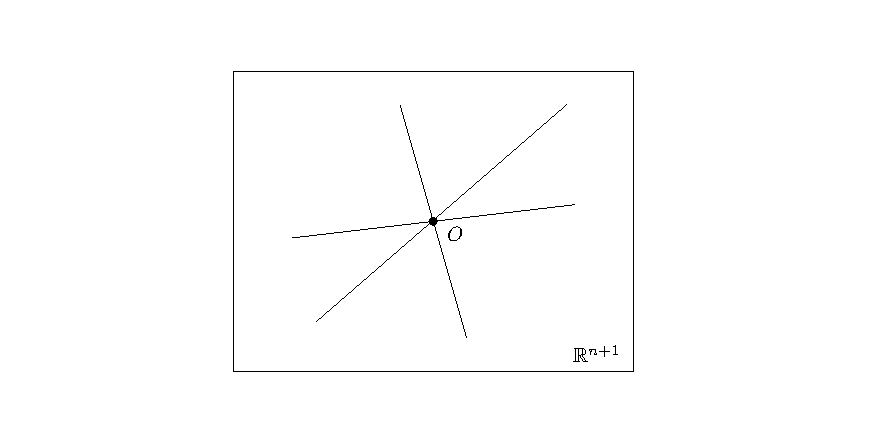
\includegraphics[width=\linewidth]{fig/fig6.pdf}
	\end{figure}

	\begin{nt}
		\
		\begin{itemize}
			\item Any non-zero $\vb x$ in $\mathbb{R}^{n+1}$ defines a point $\expval{\vb x}$ in $\RP{n}$;
			\item All lines arise in this way;
			\item Two points define the same line iff they differ by rescaling.
		\end{itemize}
	\end{nt}

	So wer can label points of $\RP{n}$ by the ratios $[x_0 : \cdots : x_n]$, called \emph{homogeneous coordinates}.

	Explicitly $[x_0 : \cdots : x_n] = [y_0 : \cdots : y_n]$ if and only if there exists $\lambda \in \mathbb{R}^*$ (meaning $\mathbb{R} \backslash \{0\}$) such that $\vb y = \lambda \vb x$.

	We can remove the rescaling ambiguity by dividing through by one of the coordinates, as long as it's non-zero.

	We thus define the following pseudo-charts. For $i = 0, \dots, n$ let 
	\[
		U_i = \{[x_0 : \cdots : x_n] : x_1 \neq 0\}
	\]
	and define a bijection $\varphi_i : U_i \to \mathbb{R}^n$ by
	\[
		\varphi_i ([x_0 : \cdots : x_n]) = \frac{1}{x_i}(x_0, \cdots, \hat{x}_i, \cdots , x_n),
	\]
	where the hat $\hat{x}_i$ denotes that the $x_i$ term is omitted.

	\begin{lem}
		These form a smooth pseudo-atlas.
	\end{lem}
	\begin{proof}
		We need to check $\varphi_i ( U_i \cap U_j)$ is open and $\varphi_j \cpf \varphi_i ^{-1}$ is smooth.

		WLOG $i = 0$ and $j = 1$, and let $\vb s$ and $\vb t$ be the local coordinates induced by $\varphi_0$ and $\varphi_1$. Then $\varphi_0 (U_0 \cap U_1) = \{s_1 \neq 0\}$, which is open.

		And on $U_0$ and $U_1$ the homogeneous coordinates are
		\[
			[1 : s_1 : \cdots : s_n] \quad \text{and} \quad [t_1 : 1 : t_2 : \cdots : t_n].
		\]
		
		So on $\{s_1 \neq 0\}$ the map $\varphi_1 \cpf \varphi_0^{-1}$ is given by
		\[
			t_1 = \frac{1}{s_1} \quad \text{and} \quad t_i = \frac{s_i}{s_1} \text{ for } i \geq 2,
		\]
		which is smooth.
	\end{proof}

	Upshot:
	\begin{itemize}
		\item $\RP{n}$ is a smooth $n$-manifold, up to checking the Hausdorff and second-countable conditions;
		\item It's second-countable because $\RP{n}$ is covered by finitely many of the pseudo-charts;
		\item Hausdorffness does not immediately follow from the criterion we gave last time: there exist pairs of points which are not contained in any common $U_i$, for example $[1:0: \cdots : 0]$ and $[0: 1 : \cdots : 1]$.
	\end{itemize}

	To remedy this we'll enlarge our pseudo-atlas, so that any two points can be put in a common pseudo-chart.

	First let us describe our existing pseudo-charts more geometrically. Let $\vb e_0, \cdots, \vb e_n$ be the standard basis of $\mathbb{R}^{n+1}$.

	\begin{itemize}
		\item $U_i = \{\text{lines complementary to the subspace }\expval{\vb e_0, \cdots, \hat{\vb e}_i, \cdots, \vb e_n}\}$;
		\item Any such line $T$ has a unique basis vector of the form \[
			\vb v = \vb e_i + a_0 \vb e_0 + \cdots + \widehat{a_i \vb e_i} + \cdots + a_n \vb e_n
		\]
		and $\varphi_i$ sends $T$ to the tuple $(a_0, \cdots, \hat{a}_i, \cdots , a_n) \in \mathbb{R}^n$;
		\item More intrinsically, we can view $\varphi_i (T)$ as the map \[
			\psi_T : \expval{\vb e_i} \to \expval{\vb e_0 , \cdots , \hat{\vb e}_i, \cdots, \vb e_n}
		\]
		\[
			\lambda \vb e_i \mapsto \lambda (a_0 \vb e_0 + \cdots + \widehat{a_i \vb e_i} + \cdots + a_n \vb e_n).
		\]
	\end{itemize}
	
	\begin{figure}[H]
		\centering
		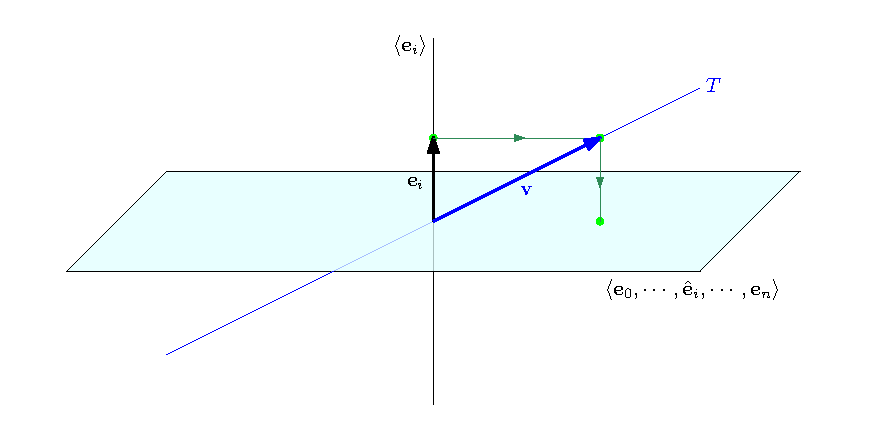
\includegraphics[width=\linewidth]{fig/fig7.pdf}
	\end{figure}

	This depends on the subspaces $\expval{\vb e_i}$ and $\expval{\vb e_0, \cdots, \hat{\vb e}_i, \cdots, \vb e_n}$ but not on any particular choice of bases.

	To generate new pseudo-charts we generalise this construction.
	\begin{itemize}
		\item Take a line $W$ in $\mathbb{R}^{n+1}$ and a complement $W^\perp$;
		\item Define $U_{W^\perp}$ in $\RP{n}$ to be $\{\text{lines complementary to }W^\perp\}$;
		\item Consider the projections $\pi_W : \mathbb{R}^{n+1} \to W$ onto $W$ along $W^\perp$ and $\pi_{W^\perp}: \mathbb{R}^{n+1}\to W^\perp$ onto $W^\perp$ along $W$;
		\item For $T$ in $U_{W^\perp}$, the map $\pi_W |_T$ gives an isomorphism $T \hme W$, so we can invert it and consider the composition \[
			\psi_T := \pi_{W^\perp} \cpf \left( \pi_W|_T \right)^{-1} : W \to W^\perp.
		\]
	\end{itemize}
	
	\begin{figure}[H]
		\centering
		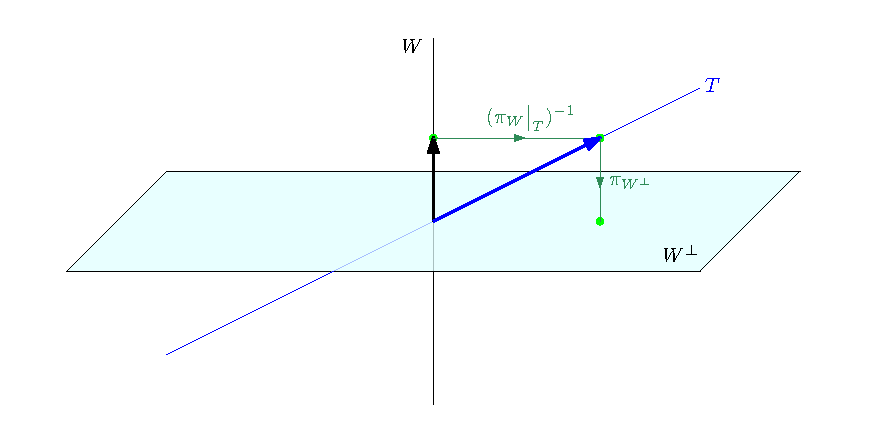
\includegraphics[width=\linewidth]{fig/fig8.pdf}
	\end{figure}

	This lifts vectors from $W$ to $T$ and then projects them onto $W^\perp$. When $W = \expval{\vb e_i}$ and $W^\perp = \expval{\vb e_0, \cdots , \hat{\vb e}_i, \cdots, \vb e_n}$ it coincides with the map $\psi_T$ we defined above.
	
	The assignment $T \mapsto \psi_T$ gives a map
	\[
		\varphi_{W,W^\perp} : U_{W^\perp} \to \mathcal{L}(W, W^\perp)
	\]
	where $\mathcal{L}(A,B)$ denotes the space of linear maps $A \to B$.

	There's also a map $\mathcal{L}(W,W^\perp) \to U_{W^\perp}$ sending $\psi$ to the image of
	\[
		W \xrightarrow{(\id_W, \psi)} W \oplus W^\perp = \mathbb{R}^{n+1}
	\]
	and this is a two-sided inverse to $\varphi_{W,W^\perp}$.
	
	\begin{lem}
		The maps $\varphi_{W,W^\perp} : U_{W^\perp} \to \mathcal{L}(W,W^\perp)$ form a smooth pseudo-atlas, enlarging the one we constructed above from the $\varphi_i$.
	\end{lem}
	\begin{proof}
		Example Sheet 1. (Can be put here when done.)
	\end{proof}

	\begin{prop}
		The above pseudo-atlas induces a Hausdorff topology on $\RP{n}$, and hence endows it with the structure of a smooth $n$-manifold.
	\end{prop}
	\begin{proof}
		For any two lines $T_1$ and $T_2$ there exists a common complement $T^\perp$, and then both lines are contained in the domain $U_{T^\perp}$ of $\varphi_{T_1, T^\perp}$.
	\end{proof}

	\begin{rmk}
		The codomain of the pseudo-chart $\varphi_{W,W^\perp}$ is $\mathcal{L}(W,W^\perp)$, which is not $\mathbb{R}^n$ but an abstract $n$-dimensional real vector space.

		To remedy this one can
		\begin{itemize}
			\item Choose a basis for each $\mathcal{L}(W,W^\perp)$ to identify it with $\mathbb{R}^n$;
			\item Or, better, choose \emph{all} bases, i.e.\ define a separate pseudo-chart \[
				\varphi_{W,W^\perp,B}: U_{W^\perp} \to \mathbb{R}^n
			\]
			for each basis $B$. Different bases give charts differing by linear (hence smooth) maps.
		\end{itemize}

		Using the same argument, from now on we allow the codomain of a (pseudo-)chart to be any abstract $n$-dimensional real vector space.
	\end{rmk}

	The space $\RP{n}$ parametrises lines, i.e.\ 1-dimensional linear subspaces, in $\mathbb{R}^{n+1}$. This has an obvious extension to a space parametrising $k$-dimensional subspaces.

	\begin{defi}
		The \emph{Grassmannian of $k$-planes in $\mathbb{R}^n$}, denoted $\Gr{k}{n}$, is the set of $k$-dimensional linear subspaces of $\mathbb{R}^n$. 
	\end{defi}

	We make this into a smooth manifold via a pseudo-atlas that generalises what we did for $\RP{n} = \Gr{1}{n+1}$.

	Construction:
	\begin{itemize}
		\item Take a $k$-dimensional subspace $W$ of $\mathbb{R}^n$ and a complement $W^\perp$;
		\item Let $U_{W^\perp} = \{\text{complementary subspaces to }W^\perp\}$;
		\item We have projection maps $\pi_W$ and $\pi_{W^\perp}$ as before, and define $\varphi_{W,W^\perp}: U_\perp \to \mathcal{L}(W,W^\perp)$ by \[
			T \mapsto \psi_T := \pi_{W^\perp} \cpf \left( \pi_W | T \right)^{-1}
		\]
		\item This has a two-sided inverse \[
			\psi \in \mathcal{L}(W, W^\perp) \mapsto \text{im}(W \xrightarrow{(\id_W, \psi)} W \oplus W^\perp = \mathbb{R}^n).
		\]
	\end{itemize}

	The overlap condition is satisfied, so we have a smooth pseudo-atlas. Hausdorff is proved as for $\RP{n}$. Second-countable follows from the fact that $\Gr{k}{n}$ can be covered by finitely many charts.

	\begin{prop}
		$\Gr{k}{n}$ is naturally a smooth manifold of dimension\\ $\dim \mathcal{L}(W,W^\perp) = k(n-k)$. 
	\end{prop}

	\begin{rmk}
		Analogously \emph{complex projective space} $\mathbb{CP}^n$ parametrises complex lines in $\mathbb{C}^{n+1}$, and the \emph{complex Grassmannian} $\mathrm{Gr}_{\mathbb{C}}(k,n)$ parametrises complex $k$-dimensional subspaces of $\mathbb{C}^n$.
	\end{rmk}

	Here transition maps are between open subsets of $\mathbb{C}^n$ or $\mathbb{C}^{k(n-k)}$, and are \emph{holomorphic}. Thus $\mathbb{CP}^n$ and $\mathrm{Gr}_{\mathbb{C}}(k,n)$ are examples of \emph{complex manifolds}, defined in the same way as smooth manifolds but with $\mathbb{R}$ and `smooth' replaced by $\mathbb{C}$ and `holomorphic'.

	\subsection{Smooth Maps} \recnr{4}

	Smoothness of maps is expressed in the local coordinates of a smooth atlas.

	Fix manifolds $X$ and $Y$ of dimensions $n$ and $m$, and smooth atlases $\{\varphi_\alpha : U_\alpha \hme V_\alpha\}_{\alpha \in \mathcal{A}}$ and $\{\psi_\beta : S_\beta \hme T_\beta\}_{\beta \in \mathcal{B}}$ on $X$ and $Y$.
	
	\begin{defi}
		A map $F : X \to Y$ between manifolds is \emph{smooth with respect to these atlases} if it's continuous and if for all $\alpha$ and $\beta$ the map
		\[
			\psi_\beta \cpf F \cpf \varphi_\alpha^{-1} : \varphi_\alpha (F^{-1} (S_\beta)) \to T_\beta
		\]
		is smooth as a map between open subsets of $\mathbb{R}^n$ and $\mathbb{R}^m$.
	\end{defi}
	\needfig{9}

	If $x_1, \cdots, x_n$ and $y_1, \cdots, y_m$ are the corresponding local coordinates, then $F$ makes the $y_i$ into functions of the $x_j$ and we are just asking that each $y_i$ has all partial derivatives with respect to the $x_j$.

	\begin{rmk}
		Continuity of $F$ means $F^{-1}(S_\beta)$ is open, so the domain of 
		\begin{equation}
			\psi_\beta \cpf F \cpf \varphi_\alpha^{-1} : \varphi_\alpha (F^{-1}(S_\beta)) \to T_\beta
			\label{eq:1.4.1}
		\end{equation}
		is open, so its smoothness makes sense.
	\end{rmk}

	\begin{lem}
		$F: X\to Y$ is smooth with respect to these atlases if and only if it's continuous and for all $p$ in $X$ there exists $U_\alpha$ containing $p$ and $S_\beta$ containing $F(p)$ such that (\ref{eq:1.4.1}) is smooth.
	\end{lem}
	\begin{proof}
		Use smoothness of the atlases plus the chain rule.
	\end{proof}

	\begin{cor}
		Smoothness of $F: X \to Y$ is independent of the choice of smooth atlases representing the smooth structures on $X$ and $Y$.
	\end{cor}
	\begin{proof}
		Reduce to the case where one atlas contains the other.
	\end{proof}

	\begin{defi}
		A map $F \to Y$ is \emph{smooth} if it's smooth with respect to some (or equivalently all) smooth atlas(es) representing the smooth structure on $X$ and $Y$.
	\end{defi}

	\begin{ex}
		\ 
		\begin{enumerate}
			\item The identity map on any manifold is smooth;
			\item Any constant map $X \to Y$ is smooth;
			\item The projections $X \times Y \to X$ and $X \times Y \to Y$ are smooth;
			\item The inclusion $S^n \hookrightarrow \mathbb{R}^{n+1}$ is smooth.
		\end{enumerate}
	\end{ex}

	We have the following basic properties.

	\begin{lem}
		\
		\begin{enumerate}
			\item A map $f: X \to \mathbb{R}$ is smooth if and only if it's a smooth function in the sense of Section \ref{sec:1.1};
			\item A map from an open subset of $\mathbb{R}^n$ to an open subset of $\mathbb{R}^m$ is smooth if and only if it's smooth in the usual multi-variable calculus sense;
			\item Smoothness is \emph{local in the source}, meaning that a map $F: X \to Y$ is smooth if and only if there exists an open cover $\{W_\gamma\}_{\gamma\in \mathcal{C}}$ of $X$ such that $F|_{W_\gamma}$ is smooth for all $\gamma$;
			\item A composition of smooth maps is smooth.
		\end{enumerate}
	\end{lem}
	
	It's helpful to have a criterion that doesn't explicitly mention the topology, for examples defined using pseudo-atlases.

	\begin{prop} \label{prop:1.41}
		A map $F: X\to Y$ is smooth if and only if there exists a cover $\{W_\gamma\}_{\gamma \in \mathcal{C}}$ of $X$, and for each $\gamma \in \mathcal{C}$ there exists elements $\alpha(\gamma) \in \mathcal{A}$ and $\beta(\gamma) \in \mathcal{B}$, such that for all $\gamma$ we have:
		\begin{enumerate}
			\item $W_\gamma$ is contained in $U_{\alpha(\gamma)}$ and $F(W_\gamma)$ is contained in $S_{\beta(\gamma)}$;
			\item $\varphi_{\alpha(\gamma)}(W_\gamma)$ is open in $V_{\alpha(\gamma)}$. [Equivalent to $W_\gamma$ being open in $X$];
			\item The map \[
				\psi_{\beta(\gamma)} \cpf F \cpf \varphi_{\alpha(\gamma)}|_{W_\gamma}^{-1} : \varphi_{\alpha(\gamma)}(W_\gamma) \to T_{\beta(\gamma)}
			\]
			is smooth.
		\end{enumerate}  
	\end{prop}
	\begin{proof}
		For the `only if' direction take $\mathcal{C} = \mathcal{A}\times \mathcal{B}$, then for $\gamma = (a,b) \in \mathcal{C}$ set $W_\gamma = U_a \cap F^{-1}(S_b), \alpha(\gamma) = a, \beta(\gamma) = b$.
		
		For the converse, the non-trivial thing to check is continuity of $F$, so tkae an open $S \subset Y$. We need to show $F^{-1}(S)$ is open in $X$, or equivalently that $F^{-1}(S) \cap W_\gamma$ is open in $X$ for all $\gamma$. This holds iff $\varphi_{\alpha(\gamma)} (F^{-1}(S)\cap W_\gamma)$ is open in $V_{\alpha(\gamma)}$ for all $\gamma$.
		
		For each $\gamma$, abbreviating $\alpha(\gamma)$ and $\beta(\gamma)$ to $\alpha$ and $\beta$ we have
		\begin{align*}
			\varphi_\alpha (F^{-1}(S) \cap W_\gamma) & = \varphi_\alpha (F^{-1}(S \cap S_\beta) \cap W_\gamma) \\
			& = \varphi_\alpha (F^{-1} (S \cap S_\beta)) \cap \varphi_\alpha(W_\gamma) \\
			& = (\psi_\beta \cpf F \cpf \varphi_\alpha^{-1})^{-1} (\psi_\beta (S)) \cap \varphi_\alpha(W_\gamma).
		\end{align*}

		This is open since $\psi_\beta(S)$ is open, $\psi_\beta \cpf F \cpf \varphi_\alpha^{-1}$ is smooth (hence continuous), and $\varphi_\alpha (W_\gamma)$ is open.
	\end{proof}

	\begin{ex}
		Viewing $\mathbb{C}^{n+1}$ as $\mathbb{R}^{2(n+1)}$, we can think of $S^{2n+1}$ as the unit sphere in $\mathbb{C}^{n+1}$. Sending a point on this sphere to the complex line through that point gives a map
		\[
			H : S^{2n+1} \to \mathbb{CP}^{n}
		\]
		called the \emph{Hopf map}. On Example Sheet 1 you will check that this is smooth using Proposition \ref{prop:1.41}.

		\needfig{11}
	\end{ex}

	\begin{defi}
		A \emph{diffeomorphism} from one manifold to another is a smooth map with a smooth two-sided inverse. Two manifolds are \emph{diffeomorphic}, written $\cong$, if there exists a diffeomorphism between them. This is obviously an equivalence relation.
	\end{defi}

	Recall from Section \ref{sec:1.1} that:
	\begin{itemize}
		\item When $n = 1,2$, or 3, every topological $n$-manifolds admits an essentially unique smooth structure.
		\item For $n \geq 4$ a topological $n$-manifold may admit many essentially different smooth structures.
	\end{itemize}

	Here `essentially unique' means `unique up to diffeomorphism', and `essentially different' means `non-diffeomorphic'.

	\begin{ex}
		$\CP{1}$ is diffeomorphic to $S^2$ via
		\[
			[z_0 : z_1] \mapsto \frac{1}{\norm{\vb z}^2} \left( 2 \bar{z}_0 z_1, \abs{z_1}^2 - \abs{z_0}^2 \right) \in S^2 \subset \mathbb{C} \oplus \mathbb{R} = \mathbb{R}^3, 
		\]
		so it makes sense to call $\CP{1}$ the \emph{Riemann sphere} and to talk about the Hopf map $S^3 \to S^2$. The conventions here are that $\CP{1}$ is viewed as $\mathbb{C} \cup \{\infty\}$ via $z \in \mathbb{C} \mapsto [1 : z]$ and $\infty \mapsto [0:1]$. Meanwhile, we put $\mathbb{C}$ inside $\mathbb{R}^3$ via $x + \mathrm{i}y \mapsto (x,y,0)$, and stereographically project it through the north pole $N = (0,0,1)$ onto $S^2 \backslash N$.  
	\end{ex}

	\begin{rmk}
		A diffeomorphism is a smooth homeomorphism but the converse is false (see Example Sheet 1).
	\end{rmk}

	\begin{lem}[Uniqueness of dimension]
		If $X$ and $Y$ are diffeomorphic non-empty manifolds then $\dim X = \dim Y$.
	\end{lem}
	\begin{proof}
		Fix a diffeomorphism $F : X \to Y$ and a point $p$ in $X$. Take charts $\varphi : U \hme V$ on $X$ about $p$ and $\psi : S \hme T$ on $Y$ about $F(p)$. By shrinking $U,V,S$ and $T$ if necessary, we may assume that $F(U)=S$.
		
		Then $G: = \psi \cpf F \cpf \varphi^{-1}$ and $H := \varphi \cpf F^{-1} \cpf \psi^{-1}$ are mutually inverse smooth maps between open subsets $V \subset \mathbb{R}^n$ and $T \subset \mathbb{R}^m$. From multivariable calculus we then have that the derivatives $\mathrm{D}_{\varphi(p)}G$ and $\mathrm{D}_{\psi(F(p))} H$ are mutually inverse linear maps between $\mathbb{R}^{\dim X}$ and $\mathbb{R}^{\dim Y}$, so $\dim X$ and $\dim Y$ must be equal.
	\end{proof}

	\subsection{Tangent Spaces} \recnr{5}
	
	The tangent space parametrises infinitesimal directions in a manifold.

	Fix an $n$-manifold $X$ and a point $p$ in $X$.

	\begin{defi}
		A \emph{curve based at $p$} is a smooth map $\gamma : I \to X$ from an open neighbourhood $I$ of $0$ in $\mathbb{R}$, satisfying $\gamma(0) = p$. We say that curves $\gamma_1 : I_1 \to X$ and $\gamma_2 : I_2 \to X$ \emph{agree to first order} if there exists a chart $\varphi : U \hme V$ about $p$ such that 
		\[
			\dv{t}\bigg|_{t=0} \varphi \cpf \gamma_1(t) = \dv{t}\bigg|_{t=0} \varphi \cpf \gamma_2 (t)
		\]
		as vectors in $\mathbb{R}^n$.
	\end{defi}
	\needfig{12}

	From now on, given a smooth real- or vector-valued function $h$ on a neighbourhood of some $t_0$ in $\mathbb{R}$, we'll write $h'(t_0)$ for
	\[
		\dv{t}\bigg|_{t = t_0} h(t).
	\]
	
	\begin{prop}
		Agreement to first order is an equivalence relation on curves based at $p$.
	\end{prop}

	\begin{proof}
		It's manifestly reflexive and symmetric. Transitivity is a consequence of the following lemma.
	\end{proof}

	\begin{lem} \label{lem:1.49}
		If $(\varphi \cpf \gamma_1)' (0) = (\varphi \cpf \gamma_2)' (0)$ holds for some chart $\varphi$ about $p$ then it holds for all such charts. 
	\end{lem}
	\begin{proof}
		Given a chart $\varphi$ about $p$, let
		\[
			\pi^\varphi_p : \{\text{curves based at } p\} \to \mathbb{R}^n
		\]
		denote the map
		\[
			\gamma \mapsto (\varphi \cpf \gamma)' (0).
		\]
		
		Now suppose $\varphi_1$ and $\varphi_2$ are two charts about $p$. We want to show that if two curves have the same image under $\pi_p^{\varphi_1}$ then they also have the same image under $\pi_p^{\varphi_2}$. To prove that this holds, note that by the chain rule we have $\pi_p^{\varphi_2} = A \cpf \pi_p^{\varphi_1}$, where $A$ is the linear map $\mathbb{R}^n \to \mathbb{R}^n$ given by the derivative of $\varphi_2 \cpf \varphi_1^{-1}$ at $\varphi_1(p)$. 
	\end{proof}

	\begin{defi}
		The \emph{tangent space to $X$ at $p$}, denoted $T_p X$, is the set of curves based at $p$ modulo agreement to first order. Elements are called \emph{tangent vectors at $p$}. We write $[\gamma]$ for the tangent vector represented by a curve $\gamma$. Intuitively this is the infinitesimal direction in which $\gamma$ passes through $p$.
	\end{defi}
	\needfig{13}

	By construction, for each chart $\varphi$ about $p$ the map $\pi_p^\varphi$ embeds $T_p X$ into $\mathbb{R}^n$. We claim that each $\pi_p^\varphi$ is in fact surjective, so induces a bijection $T_p X \to \mathbb{R}^n$. For different choices of chart these bijections differ by a linear automorphism of $\mathbb{R}^n$, namely the derivative of the transition map (called $A$ in the proof of Lemma \ref{lem:1.49}). We get the following.

	\begin{prop}
		$T_p X$ naturally carries the structure of an $n$-dimensional real vector space, in such a way that each $\pi_p^\varphi$ is a linear isomorphism.
	\end{prop}
	\begin{proof}
		The only thing left to show is that for each $\varphi$ the map $\pi_p^\varphi$ is surjective. Given a vector $\vb v \in \mathbb{R}^n$, define a curve $\gamma$ based at $p$ by $\gamma(t) = \varphi^{-1}(\varphi(p) + t \vb v)$, for all $t$ in a small open neighbourhood of $0$ in $\mathbb{R}$. By construction this satisfies $\pi_p^\varphi (\gamma) = \vb v$. 
	\end{proof}
	\needfig{14}

	\begin{defi}
		If $x_1 , \cdots, x_n$ are the local coordinates associated to the $\varphi$ then we denote by $\pdv*{x_i}$ the tangent vector $(\pi_p^\varphi)^{-1} (\vb e_i)$, where $\vb e_i$ is the $i$-th standard basis vector. We may abbreviate this to $\partial_{x_i}$ or even $\partial_i$ if the chart is clear. Intuitively it is the infinitesimal direction obtained by running at unit speed along the $x_i$-axis, i.e.\ the curve along which all other $x_j$ are constant.
	\end{defi}
	\needfig{15}

	Note that $\partial_{x_i}$ may denote a tangent vector at any point in the domain of the chart $\varphi$, and we will either be thinking of it as this whole family of vectors (a simple example of a \emph{vector field}) or we will specify at which specific point $p$ we are looking.
	
	\needfig{16}

	\begin{rmk}
		The notation $\pdv*{x_i}$ is just that: a piece of notation. We shall see shortly that it is justified by the fact that these tangent vectors can be interpreted as the obvious differential operators, and that they transform in the way the notation suggests.
	\end{rmk}

	Each vector $\partial_{x_i}$ depends on \emph{all} of the local coordinates $x_1, \cdots, x_n$, not just on $x_i$ itself. Said another way, if $y_1, \cdots, y_n$ are local coordinates associated to another chart about $p$, and if $y_i = x_i$ for some $i$, then it does not automatically follow that $\partial_{x_i} = \partial_{y_i}$. In fact, the correct expression in general (without assuming $y_i = x_i$) is the following.

	\begin{lem}
		For each $i$ we have
		\[
			\pdv{y_i} = \sum_{j = 1}^n \pdv{x_j}{y_i} \pdv{x_j}.
		\]
	\end{lem}
	\begin{proof}
		Let the $\vb x$ and $\vb y$ charts be $\varphi_1$ and $\varphi_2$. Following our earlier notation we have $\pi_p^{\varphi_2} = A \cpf \pi_p^{\varphi_1}$, so for each $i$ we get
		\begin{equation}
			\partial_{y_i} = (\pi_p^{\varphi_2})^{-1}(\vb e_i) = (\pi_p^{\varphi_1})^{-1} (A^{-1} \vb e_i).
			\label{eq:1.5.1}
		\end{equation} 

		The map $A^{-1}$ is the derivative of $\varphi_1 \cpf \varphi_2^{-1}$, which expresses the $x_j$ in terms of the $y_i$, so
		\[
			A^{-1} \vb e_i = \sum_{j=1}^n \pdv{x_j}{y_i} \vb e_j.
		\]
		
		Plugging into (\ref{eq:1.5.1}) and using linearity of $(\pi_p^{\varphi_1})^{-1}$ then gives
		\[
			\pdv{y_i} = (\pi_p^{\varphi_1})^{-1} (A^{-1} \vb e_i) = \sum_{j=1}^n \pdv{x_j}{y_i}\/(\pi_p^{\varphi_1})^{-1} (\vb e_j) = \sum_{j=1}^n \pdv{x_j}{y_i}\pdv{x_j}.
		\]
	\end{proof}

	\begin{rmk}
		If a vector $[\gamma]$ is given by $\sum_i a_i \partial_{x_i}$ then we have
		\[
			(\varphi \cpf \gamma)'(0) = \pi_p^{\varphi}(\gamma) = \sum_{i = 1}^n a_i \vb e_i.
		\]
		
		Equating components of $\vb e_i$ we obtain
		\begin{equation}
			(x_i \cpf \gamma)'(0) = a_i
			\label{eq:1.5.2}
		\end{equation}
		so the coefficients of the $\partial_{x_i}$ are the derivatives of the $x_i$ along $\gamma$.
	\end{rmk}

	\subsection{Vectors as Differential Operators} \recnr{6}

	One can differentiate functions in the direction of a given tangent vector and this gives an alternative way to construct the tangent space.

	Again fix an $n$-manifold $X$ and a point $p$ in it. Given a smooth function $f$ on a neighbourhood of $p$, and a curve $\gamma$ based at $p$, one can differentiate $f$ along $\gamma$ at $p$ to obtain a number $(f \cpf \gamma)'(0)$.
	
	\needfig{17}

	\begin{lem}
		This number depends only on the tangent vector $[\gamma]$ represented by $\gamma$. In particular, if $[\gamma] = \sum_i a_i \partial_{x_i}$ with respect to local coordinates $x_1, \cdots, x_n$ about $p$, then we have
		\[
			(f \cpf \gamma)'(0) = \sum_{i = 1}^n a_i \pdv{f}{x_i}\bigg|_{p}.
		\]
	\end{lem}

	\begin{proof}
		We'll prove
		\[
			(f \cpf \gamma)'(0) = \sum_{i=1}^n a_i \pdv{f}{x_i}\bigg|_{p}.
		\]
		
		Let $\varphi$ be the chart corresponding to the coordinates $x_i$. We then have
		\[
			(f \cpf \gamma)'(0) = \dv{t}\bigg|_{t=0} \left( (f \cpf \varphi^{-1}) \cpf (\varphi \cpf \gamma) \right) (t).
		\]
		
		The function $f \cpf \varphi^{-1}$ is simply $f$ written in terms of the $x_i$, so by the chain rule we have
		\[
			(f \cpf \gamma)'(0) = \sum_{i=i}^n \pdv{f}{x_i}\bigg|_{p} (x_i \cpf \gamma)' (0).
		\]
		
		Pugging in (\ref{eq:1.5.2}) completes the proof.
	\end{proof}

	The specific open neighbourhood of $p$ on which $f$ is defined plays no role here so it is more convenient to work with germs of function.

	\begin{defi}
		A \emph{germ of a smooth function at $p$} is the equivalence class $[(U,f)]$ of a pair $(U,f)$ comprising an open neighbourhood $U$ of $p$ and a smooth function $f: U \to \mathbb{R}$, under the equivalence relation that says $(U_1,f_1)\sim (U_2, f_2)$ if and only if there exists an open neighbourhood $V$ of $p$, contained in $U_1 \cap U_2$, such that $f_1 |_V = f_2|_V$. The \emph{space of germs at $p$}, denotes $\mathcal{O}_{X,p}$, is the set of such germs of functions. 
	\end{defi}

	\needfig{18}

	\begin{lem}
		Addition and multiplication of functions makes $\mathcal{O}_{X,p}$ into a ring (all rings are associative, commutative and unital for us). Then inclusion $\mathbb{R} \hookrightarrow \mathcal{O}_{X,p}$ of germs of constant functions further makes $\mathcal{O}_{X,p}$ into an $\mathbb{R}$-algebra (a ring equipped with a ring homomorphism from $\mathbb{R}$). It has a unique maximal ideal, $\mathfrak{m}$, given by germs of functions which vanish at $p$.
	\end{lem}

	\begin{proof}
		The first two sentences are straightforward. And $\mathfrak{m}$ is a maximal ideal since it's the kernel of a ring homomorphism to a field, namely
		\[
			\mathcal{O}_{X,p} \to \mathbb{R} \quad \text{given by} \quad [(U,f)] \mapsto f(p).
		\]
		
		To see that $\mathfrak{m}$ is unique note that any element $[(U,f)]$ of $\mathcal{O}_{X,p} \backslash \mathfrak{m}$ is invertible: since $f(p) \neq 0$ the open set $V := f^{-1}(\mathbb{R}^*)$ contains $p$, and then $[(U,f)] = [(V,f|_V)] = [(V, 1/f|_V)]^{-1}$.
	\end{proof}

	A ring with a unique maximal ideal is called a \emph{local ring}, so $\mathcal{O}_{X,p}$ is local $\mathbb{R}$-algebra. The `local' terminology is motivated by this example: you can think of a local ring as looking something like `functions defined near a point', with the maximal ideal given by `functions vanishing at the point'.

	We saw earlier that the map
	\[
		\{\text{curves based at $p$}\} \times \{\text{smooth functions on a neighbourhood of $p$}\} \to \mathbb{R}
	\]
	given by $(\gamma,f) \mapsto (f \cpf \gamma)' (0)$ depends on $\gamma$ only via $[\gamma]$. Clearly it depends only on $f$ via its germ, so defines a map
	\[
		T_p X \times \mathcal{O}_{X,p} \to \mathbb{R}.
	\]
	
	Our explicit expression for it shows that this map is bilinear, so we can view it as a linear map
	\[
		D : T_p X \to \mathcal{O}_{X,p}^{\vee}
	\]
	where $^{\vee}$ denotes the ($\mathbb{R}$-)linear dual of a vector space.

	Geometrically, $D$ sends a tangent vector to the linear operator which takes the directional derivative along the vector. In particular, $D(\partial_{x_i}) = \pdv*{x_i}$, so $D$ is injective.
	
	Clearly $D$ is far from surjective for $\dim X = n > 0$, since $\mathcal{O}_{X,p}$ is infinite-dimensional. However, for all $\vb v$ in $T_p X$ the element $D(\vb v)$ in $\mathcal{O}_{X,p}^{\vee}$ has the following property.

	\begin{lem}
		For all $f$ and $g$ in $\mathcal{O}_{X,p}$ (we are dropping the $[(U,f)]$ notation) we have
		\[
			D(\vb v) (fg) = D(\vb v)(f)\ g(p) + f(p)\ D(\vb v)(g).
		\]
		\label{lem:1.59}
	\end{lem}
	\begin{proof}
		Write $\vb v$ as $[\gamma]$ for some curve $\gamma$, and apply the product rule to the function $(fg)\cpf \gamma$.
	\end{proof}

	\begin{defi}
		Given a ring $R$, an $R$-algebra $S$, and an $S$-module $M$, an \emph{$R$-linear derivation from $S$ to $M$} is an $R$-linear map $\dd : S \to M$ such that for all $f$ and $g$ in $S$ the Leibniz rule
		\[
			\dd{(fg)} = \dd{(f)} g + f \dd{(g)}
		\]
		holds. This equality is in $M$, and $\dd{(f)}g$ denotes the module action of $g \in S$ on $\dd{(f)} \in M$ (similarly for $f \dd{(g)}$). The set of all such derivations is denoted by $\Der_R (S,M)$, and is an $R$-submodule of $\Hom_R (S,M)$.
	\end{defi}

	\begin{rmk}
		\ 
		\begin{itemize}
			\item It's the algebraic version of differential operators;
			\item Automatically $\dd{(r)} = 0$ for all $r\in R$. (Think: the derivative of a constant is zero.) This is because $\dd{(r)} = r \dd{(1)}$ and \[
				\dd{(1)} = \dd{(1 \times 1)} = \dd{(1)} \times 1 + 1 \times \dd{(1)} = 2 \dd{(1)}.
			\]
		\end{itemize}
	\end{rmk}

	Lemma \ref{lem:1.59}, i.e.\ the equality
	\[
		D(\vb v) (fg) = D(\vb v)(f)\ g(p) + f(p)\ D(\vb v)(g)
	\]
	tells us that for all $\vb v$ the element $D(\vb v)\in \mathcal{O}_{X,p}^{\vee} = \Hom_{\mathbb{R}}(\mathcal{O}_{X,p},\mathbb{R})$ is actually contained in the $\mathbb{R}$-linear subspace $\Der_{\mathbb{R}}(\mathcal{O}_{X,p},\mathbb{R})$.
	
	\begin{itemize}
		\item $R = \mathbb{R}$ and $S = \mathcal{O}_{X,p}$ is an $R$-algebra by inclusion of constants;
		\item $M = \mathbb{R}$ and is made into an $\mathcal{O}_{X,p}$-module by defining $f$ to act as $f(p)$, or more abstractly by viewing $\mathbb{R}$ as $\mathcal{O}_{X,p}/\mathfrak{m}$.
	\end{itemize}

	So the linear map $D : T_p X \to \mathcal{O}_{X,p}^{\vee}$ lands in $\Der_{\mathbb{R}}(\mathcal{O}_{X,p},\mathbb{R})$.

	\begin{prop}
		The map $D : T_p X \to \Der_{\mathbb{R}}(\mathcal{O}_{X,p}, \mathbb{R})$ is an isomorphism. So $\Der_{\mathbb{R}}(\mathcal{O}_{X,p},\mathbb{R})$ gives an alternative definition of $T_p X$ as a vector space. 
	\end{prop}

	\begin{proof}
		We saw $D$ is linear and injective, so it suffices to prove surjectivity. Suppose $\delta : \mathcal{O}_{X,p} \to \mathbb{R}$ is a derivation, and fix local coordinates $\vb x$ with $\vb x(p) = 0$. We view elements of $\mathcal{O}_{X,p}$ as functions of the $x_i$.

		Given $[(U,f)]$ in $\mathcal{O}_{X,p}$, the intuitive idea is to Taylor expand $f$ in the $x_i$. We know $\delta$ kills the constant term, and by Leibniz it also kills quadratic terms and higher. So we get
		\[
			\delta(f) = \delta \left( \sum_{i = 1}^n x_i \pdv{f}{x_i}\bigg|_{p} \right) = \sum_{i=1}^n \delta(x_i) \pdv{f}{x_i}\bigg|_{p} = \sum_{i=1}^n \delta(x_i) D(\partial_{x_i})(f).
		\]
		Hence $\delta = D(\sum_i \delta(x_i) \partial_{x_i})$ is in the image of $D$.

		To make this rigorous, fix $[(U,f)]$ and define $g : U \to \mathbb{R}$ by
		\[
			g = \begin{dcases}
				\frac{f(x_1,\cdots,x_n) - f(x_1,\cdots,x_{n-1},0)}{x_n} & \text{if }x_n \neq 0,\\
				\pdv{f}{x_n}\/(x_1, \cdots, x_n) & \text{if }x_n = 0.
			\end{dcases}
		\]
		By l'H\^opital's rule this is continuous and, inductively, smooth, so defines an element of $\mathcal{O}_{X,p}$. Letting $f_n \in \mathcal{O}_{X,p}$ be given by
		\[
			f_n (x_1, \cdots, x_n) = f(x_1, \cdots, x_{n-1}, 0),
		\]
		we have $f = f_n + x_n g$ in $\mathcal{O}_{X,p}$, and so
		\[
			\delta(f) = \delta (f_n) + \delta (x_n) g(p) + x_n (p) \delta (g) = \delta(f_n) + \delta(x_n) \pdv{f}{x_n}\bigg|_{p}.
		\]

		Iterating, we can pull out each variable in turn, and arrive at
		\[
			\delta(f) = \delta(f(p)) + \sum_{i = 1}^n \delta(x_i) \pdv{f}{x_i}\bigg|_{p}.
		\]
		
		The first term on the right-hand side vanishes since derivations kill constants, and we conclude that
		\[
			\delta = D \left( \sum_{i = 1}^n \delta(x_i) \partial_{x_i} \right)
		\]
		as claimed. So $D$ is indeed an isomorphism onto $\Der_{\mathbb{R}}(\mathcal{O}_{X,p},\mathbb{R})$.
	\end{proof}

	This result says that tangent vectors at $p$ are the same thing as derivations on $\mathcal{O}_{X,p}$, with vectors acting as the corresponding directional derivatives. Whilst our definition was more geometric, and really justifies the name `tangent vector', this derivation perspective has the advantage of marking no reference to charts.

	\subsection{Derivatives} \recnr{7}

	The derivative of a smooth map is the map it induces on curves-modulo-agreement-to-first-order.

	Fix manifolds $X$ and $Y$ and a smooth map $F: X \to Y$.

	\begin{itemize}
		\item Tangent spaces $T_p X$ and $T_q Y$ linearise $X$ and $Y$ at $p$ and $q$;
		\item The derivative of $F$ should linearise it, so should map from $T_p X$ to $T_{F(p)}Y$;
		\item Elements of $T_p X$ and $T_{F(p)}Y$ are equivalence classes of curves in $X$ and $Y$ based at $p$ and $F(p)$;
		\item There's an obvious way to use $F$ to turn curves in $X$ based at $p$ to curves in $Y$ based at $F(p)$.
	\end{itemize}

	\begin{defi}
		The \emph{derivative of $F$ at $p$}, denoted $D_p F$, is the map $T_p X \to T_{F(p)}Y$ given by $[\gamma]\mapsto [F\cpf \gamma]$. We sometimes denote $D_p F$ by $F_*$, the \emph{pushforward} by $F$ on tangent vectors. 
	\end{defi}

	\needfig{19}

	\begin{lem}
		This is well-defined and linear. If $\vb x$ and $\vb y$ are local coordinates on $X$ about $p$ and on $Y$ about $F(p)$ respectively, then viewing $F$ as a map from the $x_i$ to the $y_i$ we have
		\[
			D_p F(\partial_{x_i}) = \sum_{j=1}^m \pdv{y_j}{x_i}\bigg|_{p} \partial_{y_j}.
		\]
	\end{lem}
	\begin{proof}
		Let the $\vb x$ chart be $\varphi$. The coefficients of $\partial_{y_j}$ in $D_p F(\partial_{x_i})$ is
		\[
			\dv{t}\bigg|_{t=0} (y_j \cpf F \cpf \varphi^{-1}) (\varphi(p) + t \vb e_i) = \pdv{y_j}{x_i}.
		\]
	\end{proof}

	\begin{rmk}
		\
		\begin{itemize}
			\item This shows that the new notion of derivative coincides with the familiar multi-variable calculus version when $X$ and $Y$ are open subsets of $\mathbb{R}^m$ and $\mathbb{R}^n$ and we take the standard coordinates;
			\item For a curve $\gamma$ based at $p$ we can write $[\gamma]$ as $D_0 \gamma (\partial_t)$, where $t$ is the standard coordinate on the domain of $\gamma$.
		\end{itemize}
	\end{rmk}

	\needfig{20}

	With our new notion of derivative the chain rule is tautological.

	\begin{prop}[Chain rule]
		If $F: X \to Y$ and $G : Y \to Z$ are smooth maps between manifolds then $G \cpf F$ is also smooth and for all $p$ in $X$ we have $D_p(G \cpf F) = D_{F(p)}G\cpf D_p F$.
	\end{prop}
	\begin{proof}
		For all $[\gamma]$ in $T_p X$ we have
		\[
			D_p(G\cpf F) ([\gamma]) = [(G\cpf F)\cpf \gamma] = [G\cpf(F\cpf \gamma)] = D_{F(p)}G \cpf D_p F([\gamma]).
		\]
	\end{proof}

	The definition can be reformulated in terms of derivations:
	\begin{itemize}
		\item Given a germ $[(U,f)] \in \mathcal{O}_{Y,F(p)}$ there is an induced germ $[(F^{-1}(U), f\cpf F)] \in \mathcal{O}_{X,p}$ (this is well-defined);
		\item We get a map $F^* : \mathcal{O}_{Y,F(p)} \to \mathcal{O}_{X,p}$, called \emph{pullback by $F$};
		\item This is obviously $\mathbb{R}$-linear so has a dual map \[
			(F^*)^{\vee} : \mathcal{O}_{X,p}^{\vee} \to \mathcal{O}_{Y,F(p)}^{\vee}
		\]
		\item Since $F^*$ is moreover a homomorphism of $\mathbb{R}$-algebras (an $\mathbb{R}$-linear ring homomorphism), the map $(F^*)^{\vee}$ sends the subspace \[
			\Der_{\mathbb{R}}(\mathcal{O}_{X,p},\mathbb{R}) \subset \mathcal{O}_{X,p}^{\vee} \quad \text{to} \quad \Der_{\mathbb{R}}(\mathcal{O}_{Y,F(p)},\mathbb{R}) \subset \mathcal{O}_{Y,F(p)}^{\vee}
		\]
		\item These subspaces are identified with $T_p X$ and $T_{F(p)}Y$ by the map $D$ which sends tangent vectors to directional derivatives. 
		
		\begin{center}
			\begin{tikzcd}
				T_p X \arrow[r, "D_p F"] \arrow[d, "D"', "\sim"] & T_{F(p)} Y \arrow[d, "\sim"', "D"]\\
				\Der_{\mathbb{R}}(\mathcal{O}_{X,p},\mathbb{R}) \arrow[r, "(F^*)^{\vee}"] & \Der_{\mathbb{R}}(\mathcal{O}_{Y,F(p)},\mathbb{R})
			\end{tikzcd}
		\end{center}
	\end{itemize}

	\begin{lem}
		The diagrams commutes, i.e.\ $D \cpf D_p F = (F^*)^{\vee} \cpf D$.
	\end{lem}
	\begin{proof}
		For all $[\gamma]$ in $T_p X$, and all $f$ in $\mathcal{O}_{Y,F(p)}$, we have
		\[
			D(D_p F([\gamma])) (f) = D([F \cpf \gamma]) (f) = \left( f \cpf (F \cpf \gamma) \right)' (0).
		\]
		
		Using the obvious associativity, this becomes
		\[
			\left( (f \cpf F) \cpf \gamma \right)' (0) = D([\gamma]) (F^* f) = (F^*)^{\vee} \left( D([\gamma]) \right) (f).
		\]
		
		This means that
		\[
			D(D_p F([\gamma])) = (F^*)^{\vee} (D([\gamma]))
		\]
		for all $[\gamma]$, which is exactly what we want.
	\end{proof}

	Geometrically this just says that if you have a tangent vector $\vb v$ in $T_p X$ and a function germ $f$ in $\mathcal{O}_{Y,F(p)}$ then you can either pushforward $\vb v$ to $T_{F(p)}Y$ and differentiate $f$ along $F_* \vb v$, or pullback $f$ to $\mathcal{O}_{X,p}$ and differentiate $F^* f$ along $\vb v$, and these give the same answer. 

	\subsection{Immersions, Submersions and Local Diffeomorphisms} \recnr{8}

	If the derivative of a smooth map is injective, surjective, or an isomorphism, then the map has a simple local description.

	First recall the following result from multi-variable calculus.

	\begin{thm}[Inverse function theorem]
		If $G : V \to T$ is a continuously differentiable function between open subsets of $\mathbb{R}^n$, whose derivative at a point $p \in V$ is a linear isomorphism $\mathbb{R}^n \to \mathbb{R}^n$, then there exists open neighbourhoods $V'$ and $T'$ of $p$ and $G(p)$ respectively such that $G\big|_{V'}$ is a bijection $V' \to T'$ and the inverse is also continuously differentiable. 
	\end{thm}

	\needfig{21}

	\begin{proof}
		See Rudin's \emph{Principles of Mathematical Analysis}:\ Theorem 9.24 in the third edition.
	\end{proof}

	\begin{cor}
		If, under the same hypotheses, $G$ is actually smooth then so is the inverse.
	\end{cor}

	\begin{proof}
		The derivative $D(G^{-1})$ of the inverse is given by $(DG)^{-1}$, and the entries of the latter have explicit expressions in terms of the partial derivatives of $G$, which can be further differentiated arbitrarily many times.
	\end{proof}

	From now on fix manifolds $X$ and $Y$ of dimensions $n$ and $m$ respectively, and a smooth map $F: X\to Y$.

	\begin{defi}
		Given a point $p$ in $X$, say $F$ is
		\begin{itemize}
			\item An \emph{immersion at $p$} if $D_p F$ is injective;
			\item A \emph{submersion at $p$} if $D_p F$ is surjective;
			\item A \emph{local diffeomorphism at $p$} if $D_p F$ is an isomorphism. 
		\end{itemize}

		These require $n \leq m, n \geq m,$ and $n = m$ respectively. The points $p$ at which $F$ is a submersion are called \emph{regular points of $F$}. The non-regular points are called \emph{critical points of $F$}.
	\end{defi}

	The name `local diffeomorphism' is justified by the following.

	\begin{prop}
		If $D_p F$ is an isomorphism then there exists an open neighbourhood $U$ of $p$ in $X$ and an open neighbourhood $S$ of $F(p)$ in $Y$ such that $F\big|_{U}$ is a diffeomorphism $U \to S$.
		\label{prop:1.71}
	\end{prop}
	\begin{proof}
		Pick charts $\varphi : U \hme V$ and $\psi : S \hme T$ about $p$ and $F(p)$ respectively. By shrinking the first chart if necessary we may assume that $F(U)\subset S$. Now apply the inverse function theorem (actually the `smooth' corollary) to
		\[
			G : = \psi \cpf F \cpf \varphi^{-1} : V \to T.
		\]
		
		We obtain open subsets $V' \subset V$ and $T' \subset T$ such that $G\big|_{V'}$ is a diffeomorphism $V' \to T'$. Replace $U$ with $\varphi^{-1}(V')$ and $S$ with $\psi^{-1}(T')$ to get the result.
	\end{proof}

	\begin{ex}
		The map $\mathbb{R}_{>0} \times \mathbb{R} \to \mathbb{R}^2$ given by $(r,\theta)\mapsto (r \cos \theta, r \sin \theta)$ is a local diffeomorphism at every point. So if we restrict its domain to $\mathbb{R}_{>0} \times (\theta_0 ,\theta_0 + 2 \pi)$ for some $\theta_0$, to make it injective, then it gives a diffeomorphism
		\[
			\mathbb{R}_{>0} \times (\theta_0 ,\theta_0 + 2 \pi) \hme \mathbb{R}^2 \backslash \{(r \cos \theta_0 , r \sin \theta_0): r \in \mathbb{R}_{\geq 0}\}.
		\]
		The inverse gives a polar coordinate chart, without explicitly inverting any trig functions.
	\end{ex}

	\begin{ex}
		The map $S^n \to \RP{n}$ that sends a point $p$ in $S^n$ to the line $\mathbb{R} p $ through $p$ is a local diffeomorphism. Globally it is $2 : 1$ since both $p$ and $-p$ represent the same line.
	\end{ex}

	We just proved Proposition \ref{prop:1.71}. This lets us construct charts on $X$ from charts on $Y$ and vice versa:
	\begin{itemize}
		\item By shrinking $U$ and $S$ if necessary we may assume that $S$ is the domain of some chart $\psi : S \hme T$. In fact, the $S$ we constructed in the proof already has this property. Then $\psi \cpf F : U \hme T$ defines a chart about $p$ on $X$;
		\item By shrinking so that $U$ is the domain of a chart $\varphi: U \hme V$ then $\varphi \cpf \left( F\big|_U \right)^{-1} : S \hme V$ gives a chart about $F(p)$ on $Y$. 
	\end{itemize}

	The upshot is the following:

	\begin{lem}
		If $F$ is a local diffeomorphism at $p$, and $x_1, \cdots, x_n$ are local coordinates on $X$ about $p$, then there exists local coordinates $y_1, \cdots, y_n$ on $Y$ about $F(p)$ such that in terms of $\vb x$ and $\vb y$ the map $F$ is given by the identity map on $\mathbb{R}^n$. In other words $\vb y \cpf F = \vb x$. Similarly, given coordinates $\vb y$ about $F(p)$ there exists coordinates $\vb x$ about $p$ such that $\vb y \cpf F = \vb x$.
	\end{lem}
	\begin{proof}
		If $\varphi$ is the chart defining the coordinates $\vb x$ then take $\vb y$ to be the coordinates associated to the chart $\varphi \cpf \left( F \big|_U \right)^{-1}$ constructed just above. Similarly, if the $\vb y$ coordinates are associated to $\psi$ then take $\vb x$ to be the coordinates associated to $\psi \cpf F$. 
	\end{proof}

	There are also nice local forms for immersions and submersions.

	\begin{lem}
		Suppose $F$ is an immersion at $p$ and $x_1, \cdots, x_n$ are local coordinates about $p$. Then there exists local coordinates $y_1, \cdots, y_m$ about $F(p)$ such that, in terms of $\vb x$ and $\vb y$, $F$ is given on a neighbourhood of $p$ by the inclusion
		\[
			\mathbb{R}^n = \mathbb{R}^n \oplus 0 \hookrightarrow \mathbb{R}^n \oplus \mathbb{R}^{m-n} = \mathbb{R}^m.
		\]
		In other words $\vb y \cpf F = (x_1, \cdots, x_n, 0, \cdots, 0)$.

		Similarly, if $F$ is a submersion at $p$ then given local coordinates $\vb y$ about $F(p)$ there exists local coordinates $\vb x$ about $p$ in which $F$ is given by the projection
		\[
			\mathbb{R}^n = \mathbb{R}^m \oplus \mathbb{R}^{n-m} \twoheadrightarrow \mathbb{R}^m,
		\]
		i.e.\ $\vb y \cpf F = (x_1, \cdots, x_m)$.
	\end{lem}
	\begin{proof}
		The idea is to bulk up the domain or the codomain in order to make $F$ a local diffeomorphism. We'll do the submersion case but the immersion case is similar.

		We're given coordinates $\vb y$ on $Y$ about $F(p)$, and these correspond to some chart $\psi : S \hme T$. Take an arbitrary chart $\varphi : U \hme V$ on $X$ about $p$. Replacing $F$ with $\psi \cpf F \cpf \varphi^{-1}$ we may assume that $X$ and $Y$ are open subsets of $\mathbb{R}^n$ and $\mathbb{R}^m$. Their tangent spaces are then also identified with $\mathbb{R}^n$ and $\mathbb{R}^m$.

		We want a change of coordinates $\chi$ on $\mathbb{R}^n$ about $p$ so that
		\[
			F \cpf \chi^{-1} \quad \text{is projection} \quad \mathbb{R}^n = \mathbb{R}^m \oplus \mathbb{R}^{n-m} \twoheadrightarrow \mathbb{R}^m.
		\]
		The local coordinates associated to $\chi \cpf \varphi$ then give the desired $\vb x$.

		Now we
		\begin{itemize}
			\item Have $F : X \subset \mathbb{R}^n \to Y \subset \mathbb{R}^m$ smooth, $D_p F$ surjective;
			\item Want $\chi$ such that $F \cpf \chi^{-1}$ is projection $\mathbb{R}^n \twoheadrightarrow \mathbb{R}^m$.
		\end{itemize}

		Let $K$ denote the kernel of $D_p F : T_p X = \mathbb{R}^n \to T _{F(p)} Y = \mathbb{R}^m$. Pick an arbitrary linear projection $\pi : \mathbb{R}^n \to \mathbb{R}^{n-m}$ which induces an isomorphism $K \to \mathbb{R}^{n-m}$. Now consider the map
		\[
			\chi : X \to Y \times \mathbb{R}^{n-m} \quad \text{given by} \quad (F,\pi).
		\]
		This is smooth, and its derivative at $p$ is  
		\[
			(D_p F, \pi) : T_p X = \mathbb{R}^n \to T _{F(p)}Y \oplus \mathbb{R}^{n-m} = \mathbb{R}^m \oplus \mathbb{R}^{n-m} = \mathbb{R}^n,
		\]
		which is an isomorphism. So $\chi$ gives a change of coordinates about $p$, and by construction $F \cpf \chi^{-1}$ is projection onto the first $m$ components.
	\end{proof}

	\subsection{Submanifolds} \recnr{9}

	A subset of an $n$-manifold naturally inherits the structure of an $(n-k)$-manifold if it is defined locally by the vanishing of $k$ local coordinates.

	Fix an $n$-manifold $X$.

	\begin{defi}
		A subset $Z \subset X$ is a \emph{submanifold (of codimension $k$)} if for all $p$ in $Z$ there exists an open neighbourhood $U$ of $p$ in $X$, and local coordinates $x_1, \cdots, x_n$ defined on $U$, such that $Z \cap U$ is given by $x_1 = \cdots = x_k = 0$.
	\end{defi}

	\needfig{22}

	\begin{ex}
		The unit circle in $\mathbb{R}^2$ is a submanifold of codimension 1: about each point there are polar coordinates $(r,\theta)$, and if we take $(x_1,x_2) = (r-1,\theta)$ then the circle is given by $x_1 = 0$.
	\end{ex}

	\begin{rmk}
		Note we require the existence of nice coordinates about each $p$ in $Z$, \emph{not} each $p$ in $X$. For instance, the set
		\[
			Z : = \{(x,0): x\neq 0\} \subset \mathbb{R}^2
		\]
		is a submanifold of $\mathbb{R}^2$, even though near the origin $Z$ is not described by the vanishing of a local coordinate function.
	\end{rmk}
	\needfig{23}

	Fix a submanifold $Z \subset X$ of codimension $k$.

	\begin{itemize}
		\item $Z$ carries a subspace topology, which is Hausdorff and second-countable because $X$ is;
		\item For each point $p$ in $Z$ there exists local coordinates $\vb x$ about $p$ such that $Z = \{x_1 = \cdots = x_k = 0\}$. Then $x _{k+1}, \cdots, x_n$ form local coordinates on a neighbourhood of $p$ in $Z$, i.e.\ they define a chart of $Z$ about $p$;
		\item The transition functions between different charts constructed in this way are smooth, because the original transition functions on $X$ were smooth. So doing this for all $p,U$ and $\vb x$, we obtain a smooth atlas on $Z$.
	\end{itemize}

	Equivalent atlases on $X$ induce equivalent atlases on $Z$ so we get the following.

	\begin{prop}
		A codimension-$k$ submanifold $Z \subset X$ is naturally an $(n-k)$-manifold.
	\end{prop}

	\begin{ex}
		An open subset $W \subset X$ is a codimension-0 submanifold and thus inherits an $n$-manifold structure. This agrees with the manifold structure we defined earlier on open subsets.
	\end{ex}

	Finding nice local coordinates about each point of $Z \subset X$ is fiddly. But there is a much easier way to check that $Z$ is a submanifold.

	Fix an $m$-manifold $Y$ and a smooth map $F: X \to Y$.

	\begin{defi}
		A point $q$ in $Y$ is called a \emph{regular value} if every point $p$ in $F^{-1}(q)$ is a regular point, i.e.\ $D_p F$ is surjective for all such $p$. All points in $Y$ that are not regular values are \emph{critical values}.
	\end{defi}
	\needfig{24}

	\begin{prop}
		If $q \in Y$ is a regular value, then $F^{-1}(q)$ is a codimension-$m$ submanifold of $X$.
	\end{prop}
	\begin{proof}
		For each $p \in F^{-1}(q)$ we know that $F$ is a submersion at $p$, so there exists local coordinates $\vb x$ about $p$ and $\vb y$ about $q$ such that
		\[
			\vb y \cpf F = (x_1, \cdots, x_m).
		\]
		If we translate the local coordinates so that $\vb y(q) = 0$, then on the domain of $\vb x$ we have $F^{-1}(q)$ is given by $x_1 = \cdots = x_m = 0$.
	\end{proof}

	Intuitively, the point $q$ is defined by the vanishing of $m$ local coordinate functions on $Y$, and then $Z$ is defined by the vanishing of their pullbacks under $F$.

	\begin{ex}
		Define $F : \mathbb{R}^2 \to \mathbb{R}$ by $F(x,y) = xy$. The point $0\in \mathbb{R}$ is a critical value, but all non-zero real numbers are regular values. So for $c\neq 0$ the set $F^{-1}(c) = \{xy = c\}$ is a smooth 1-manifold. The set $F^{-1}(0)$ meanwhile fails to be a manifold at the origin.
		
		\needfig{25}
	\end{ex}

	\begin{rmk}
		The pre-image of a critical value does not necessarily fail to be a submanifold of the expected dimension. For example, 0 is a critical value of $F : \mathbb{R}^2 \to \mathbb{R}$ given by $F(x,y) = x^2$. But $F^{-1}(0)$ is still a codimension-1 submanifold. 
	\end{rmk}

	\begin{ex}
		Let $F : \mathbb{R}^{n+1} \to \mathbb{R}$ be the smooth map given by $F(\vb x) = \norm{\vb x}^2$. The point $1 \in \mathbb{R}$ is a regular value, so $S^n$ is a codimension-1 submanifold of $\mathbb{R}^{n+1}$. We'll see shortly that the induced smooth structure on $S^n$ coincides with that constructed by stereographic projection.
	\end{ex}

	\begin{ex}
		The space $\mathcal{L}(\mathbb{R}^n , \mathbb{R}^n)$ is a manifold of dimension $n^2$. The map $\det$ defines a smooth function on it, so $\GL(n, \mathbb{R}) = \det^{-1}(\mathbb{R}^*)$ is an open subset and hence inherits a manifold structure. 
	\end{ex}

	\begin{clm*}
		1 is a regular value of $\det : \GL(n, \mathbb{R}) \to \mathbb{R}$, so its pre-image $\SL(n, \mathbb{R})$ is a smooth manifold of dimension $n^2 - 1$. 
	\end{clm*}

	\begin{proof}
		Take an arbitrary $A \in \SL(n,\mathbb{R})$ and consider the curve
		\[
			\gamma : t \mapsto e^t A
		\]
		in $\GL(n,\mathbb{R})$ based at $A$. We have
		\[
			D_A \det([\gamma]) = [\det \cpf \gamma] = [t \mapsto e ^{nt}] = n \partial_x \in T_1 \mathbb{R}
		\]
		where $x$ is the standard coordinate on $\mathbb{R}$. This vector is non-zero so $D_A \det$ is surjective, and we're done.
	\end{proof}

	\begin{ex}
		Let $S \subset \mathcal{L}(\mathbb{R}^n, \mathbb{R}^n)$ denote the linear subspace of symmetric matrices, of dimension $n(n+1)/2$, and consider the smooth map $F: \mathcal{L}(\mathbb{R}^n, \mathbb{R}^n) \to S$ given by $F(A) = A^T A$. The identity matrix $I \in S$ is a regular value so the orthogonal group $\Og(n) = F^{-1}(I)$ is naturally a submanifold of $\mathcal{L}(\mathbb{R}^n,\mathbb{R}^n)$ of dimension $n(n-1)/2$.  
	\end{ex}

	In order to use this criterion to produce submanifolds, we need regular values to be plentiful. Fortunately, this is the case.

	\begin{thm}[Sard's theorem]
		The set of critical values has measure 0 in $Y$. More precisely, given any chart $\psi: S \hme T$ on $Y$, the set
		\[
			\psi(S \cap \{\text{critical values of }F\}) \subset T \subset \mathbb{R}^m
		\]
		has measure 0 with respect to the Lebesgue measure on $\mathbb{R}^m$.
	\end{thm}
	\begin{proof}
		See Lee's \emph{Introduction to Smooth Manifolds}:\ Theorem 6.10 in the second edition, or Nicolaescu's \emph{Lectures on the Geometry of Manifolds}:\ Theorem 2.1.18 in the September 9, 2018 version.
	\end{proof}

	The measure zero formulation is not important for most purposes. Usually the following corollary is enough, and this will be what we mean if we say `by Sard's theorem'.

	\begin{cor}
		The regular values of $F$ are dense in $Y$. In particular, $F$ has at least one regular value.
	\end{cor}

	\begin{rmk}
		Sard's theorem guarantees the existence of regular values, but \emph{not} regular points. For example, if $X$ and $Y$ are non-empty and of positive dimension, and the map $F: X \to Y$ is constant, then every $p$ in $X$ is a critical point. But every $q$ in $Y \backslash F(X)$ is vacuously a regular value. Geometrically, although the set $C$ of critical points in $X$ may be very large, its image in $Y$ is small because $DF$ fails to be surjective at these points.
	\end{rmk}
	\needfig{26}

	\subsection{Embeddings} \recnr{10}

	Inclusions of submanifolds are smooth immersions that are homeomorphisms onto their images.

	Fix an $n$-manifold $X$ and a codimension-$k$ submanifold $Z \subset X$. Let $\iota : Z \to X$ be the inclusion. First we prove its basic properties.

	\begin{lem}
		The map $\iota$ is a smooth immersion which is a homeomorphism onto its image (equipped with the subspace topology).
		\label{lem:1.91}
	\end{lem}

	\begin{proof}
		About each $p \in Z$ we have local coordinates $\vb x$ on $X$ such that $Z$ is $x_1 = \cdots = x_k = 0$ and $x _{k+1}, \cdots, x_n$ are coordinates on $Z$. In these coordinates $\iota$ is $(x _{k+1}, \cdots, x_n) \mapsto (0,\cdots,0,x _{k+1},\cdots,x_n)$, so it's a smooth immersion. It's automatically a homeomorphism onto its image because $Z$ was given the subspace topology.
	\end{proof}

	\begin{lem}
		Post-composition with $\iota$ gives a bijection
		\[
			\{\text{smooth maps to }Z\} \underset{\iota \cpf -}{\hme} \{\text{smooth maps to $X$ with image contained in $Z$}\}.
		\]
		\label{lem:1.92}
	\end{lem}
	\begin{proof}
		Ignoring smoothness, the map $\iota \cpf -$ induces a bijection.
		\[
			\{\text{all maps to }Z\} \hme \{\text{all maps to $X$ with image contained in $Z$}\}
		\]
		since $\iota$ is injective. It preserves smoothness since $\iota$ is smooth.

		Now suppose $Y$ is a manifold and $F : Y \to Z$ is a map such that $\iota \cpf F$ is smooth. We need to show $F$ is smooth. So take coordinates $\vb x$ about an arbitrary point $p$ in the image of $F$ such that locally $Z$ is $\{x_1 = \cdots = x_k = 0\}$. Letting $\vb x' = (x _{k+1}, \cdots, x_n)$, we are given that $\vb x \cpf F$ is smooth and need to show that $\vb x' \cpf F$ is smooth. This follows immediately from the fact that the map $\vb x \mapsto \vb x'$ is smooth.
	\end{proof}

	We'll use this to formulate the converse to Lemma \ref{lem:1.91}.

	\begin{prop}
		Suppose $Y$ is an $m$-manifold and $F : Y \to X$ is a smooth immersion which is a homeomorphism onto its image. Then the image of $F$ is a submanifold $Z$ of $X$ of codimension $k := n - m$ and the smooth map $\bar{F} : Y \to Z$ induced by $F$ via Lemma \ref{lem:1.92} is a diffeomorphism.
	\end{prop}
	\begin{proof}
		First assume that the image of $F$ is a codimension-$(n-m)$ submanifold $Z$, and let $\iota : Z \hookrightarrow X$ be the inclusion. We have $\iota \cpf \bar{F} = F$, which we are assuming is an immersion. By the chain rule $\bar F$ is then also an immersion, and so by dimension it is a local diffeomorphism. Hence $\bar F$ locally has a smooth inverse, and since it's bijective $Y \to Z$ these local inverses glue together to give a global smooth inverse. Hence $\bar F$ is a diffeomorphism.

		It remains to show that $F(Y) \subset X$ is a codimension-$(n-m)$ submanifold, so take $q \in Y$ and let $p = F(q)$. Since $F$ is an immersion at $q$ there exist local coordinates $\vb y$ on a neighbourhood $S$ of $q$ in $Y$ and $\vb x$ on a neighbourhood $U$ of $p$ in $X$ such that $\vb x \cpf F = (\vb y, 0, \cdots, 0)$. Suppose we can find an open neighbourhood $U'$ of $p$ in $U$ such that $F(Y)\cap U' = F(S)\cap U'$. Then $\vb x$ defines coordinates on $U'$ and we have
		\[
			F(Y)\cap U' = \{x _{m+1} = \cdots = x_n = 0\}\cap U',
		\]
		which is what we want (i.e.\ $F(Y)$ is locally given by the vanishing of $n-m$ local coordinate functions). So it suffices to find such a $U'$.
		
		Since $F$ is a homeomorphism onto its image, the set $F(S)$ is open in $F(Y)$. Hence there exists an open neighbourhood $W$ of $p$ in $X$ such that $F(S)= F(Y)\cap W$. Taking $U' = W \cap U$ gives the result: we have
		\[
			F(Y)\cap U' = (F(Y)\cap W)\cap U = (F(S)\cap W)\cap U = F(S)\cap U'.
		\]
	\end{proof}

	\begin{prop}
		The stereographic projection definition of $S^n$ is diffeomorphic to the definition as a submanifold of $\mathbb{R}^{n+1}$.
	\end{prop}

	\begin{proof}
		Take the stereographic projection definition of $S^n$, and let $F: S^n \to \mathbb{R}^{n+1}$ be the inclusion map. This is a homeomorphism onto the unit sphere (since $S^n$ was given the subspace topology), so we are left to show it's a smooth immersion. To do this we just need to show that $F \cpf \varphi _{\pm}^{-1}$ is a smooth immersion $\mathbb{R}^n \to \mathbb{R}^{n+1}$, where
		\[
			\varphi_\pm : (x_0, \cdots, x_n) \in S^n \backslash \{(\pm 1, 0, \cdots, 0)\} \mapsto \frac{1}{1 \mp x_0} (x_1, \cdots, x_n)\in \mathbb{R}^n
		\]
		are the two charts. This can be checked using the explicit expression
		\[
			F \cpf \varphi_\pm^{-1} (\vb y) = \frac{1}{\norm{\vb y}^2 + 1} \left( \pm (\norm{\vb y}^2 - 1),2 \vb y \right).
		\]
	\end{proof}

	\begin{defi}
		An \emph{embedding} is a smooth immersion which is a homeomorphism onto its image. We've shown that submanifolds are precisely the images of embeddings. An \emph{immersed submanifold} is the image of an immersion, we won't use this notion.
	\end{defi}

	Our definition of manifold seems to allow more general objects than submanifolds of $\mathbb{R}^N$, but the following remarkable result holds.

	\begin{thm}[Whitney embedding theorem]
		Any $n$-manifold $X$ can be realised as a submanifold of $\mathbb{R}^{2n}$.
	\end{thm}

	\begin{proof}
		The weaker statement in which $2n$ is replaced by $2n + 1$ is proved in Lee's book:\ Theorem 6.15 in the second edition. The full statement appears in Whitney's paper \emph{The self-intersections of a smooth $n$-manifold in $2n$-space}, published in \emph{Ann.\ of Math.}, 1944.
	\end{proof}


	\subsection{Transversality} \recnr{11}

	The intersection of two submanifolds is a submanifold if they are transverse.

	Fix an $n$-manifold $X$, and submanifolds $Z_1$ and $Z_2$ of codimensions $k_1$ and $k_2$.

	\begin{itemize}
		\item Locally each $Z_i$ is cut out by $k_i$ equations;
		\item So roughly one expects that $Z_1 \cap Z_2$ is cut out by $k_1 + k_2$ equations and hence is a submanifold of $X$ of codimension $k_1 + k_2$;
		\item For this to work the equations must be suitably independent.
	\end{itemize}

	\begin{ex}
		If the equations are the same, so $Z_1 = Z_2$, then $Z_1 \cap Z_2$ is a submanifold but of codimension $k_1 = k_2$.
	\end{ex}

	\begin{ex}
		In general $Z_1 \cap Z_2$ isn't even a submanifold, e.g.\ if
		\[
			Z_1 = \{z=0\} \subset \mathbb{R}^3 \quad \text{and} \quad Z_2 = \{z = y^2 - x^2\}.
		\]
		\needfig{27}
	\end{ex}

	The easiest way to ensure that the equations are independent is to ask that their linearisations are linearly independent, and this is precisely what transversality does.

	\begin{itemize}
		\item Near a point $p \in Z_1 \cap Z_2$ the linearisation of $X$ is $T_p X$;
		\item The linearisation of $Z_i$ is the subspace $T_p Z_i \subset T_p X$;
		\item The linearisation of the $k_i$ equations cutting out $Z_i$ form a basis for the space of linear equations that cut out $T_p Z_i$ in $T_p X$;
		\item In other words, they form a basis for the annihilator $(T_p Z_i)^\circ$ of $T_p Z_i$, inside the dual space $(T_p X)^{\vee}$;
		\item The condition that the linear equations for $Z_1$ and $Z_2$ are independent then says that $(T_p Z_1)^\circ \cap (T_p Z_2)^\circ = 0$, which is equivalent to $T_p Z_1 + T_p Z_2 = T_p X$.  
	\end{itemize}
	\begin{defi}
		The submanifold $Z_1$ and $Z_2$ in $X$ are \emph{transverse}, denoted $Z_1 \pitchfork Z_2$, if for all $p \in Z_1 \cap Z_2$ we have $T_p Z_1 + T_p Z_2 = T_p X$.
	\end{defi}

	\begin{ex}
		If $Z_1$ and $Z_2$ are disjoint then they're vacuously transverse. If $k_1 + k_2 > n$ then $Z_1 \pitchfork Z_2$ if and only if they're disjoint.
	\end{ex}

	\begin{ex}
		Affine subspaces of $\mathbb{R}^n$ are transverse iff their intersection is an affine subspace of the expected dimension. E.g.\ in $\mathbb{R}^3$
		\begin{itemize}
			\item Two affine lines are transverse iff they are disjoint;
			\item An affine line is transverse to a plane iff it's not contained in it;
			\item A point is transverse to $\mathbb{R}^3$ but is only transverse to a proper subspace if they're disjoint.
		\end{itemize}
	\end{ex}
	\begin{rmk}
		Transversality should be viewed as the `generic' way in which submanifolds meet, meaning that any two submanifolds can be made transverse by a small perturbation. (C.f. Sard.)
	\end{rmk}

	The point of the definition was so that the following result holds.

	\begin{prop}
		If $Z_1$ and $Z_2$ are transverse then $Z_1 \cap Z_2$ is a submanifold of $X$ of codimension $k_1 + k_2$. It is also a codimension-$k_2$ submanifold of $Z_1$ and a codimension-$k_1$ submanifold of $Z_2$.
		\label{prop:1.103}
	\end{prop}

	\begin{ex}
		The line $y = c$ in $\mathbb{R}^2$ is transverse to the unit circle $S^1$ iff $c \neq \pm 1$. Even in these non-transverse cases the intersection is a 0-manifold. Note that as $c$ varies the number of points in $\{y=c\}\cap S^1$ is locally constant but jumps at $c = \pm 1$.
	\end{ex}

	We'll prove Proposition \ref{prop:1.103} by showing that if $Z_1$ and $Z_2$ meet transversely at $p$ (meaning $p$ lies in $Z_1 \cap Z_2$ and $T_p Z_1 + T_p Z_2 = T_p X$) then there exist nice local coordinates about $p$.

	\begin{lem}
		If $Z_1$ and $Z_2$ meet transversely at $p$ then there exist local coordinates $x_1, \cdots, x_n$ about $p$ in which $Z_1$ is given by $x_1 = \cdots = x _{k_1} = 0$ and $Z_2$ is given by $x _{k_1 + 1} = \cdots = x _{k_1 + k_2} = 0$.
	\end{lem}

	\begin{proof}
		Let $\vb a$ and $\vb b$ be local coordinates on a neighbourhood $U$ of $p$ in which $Z_1$ is $a_1 = \cdots = a _{k_1} = 0$ and $Z_2$ is $b_1 = \cdots = b _{k_2} = 0$. Consider
		\[
			F: U \to \mathbb{R} ^{k_1 + k_2} \quad \text{given by} \quad (a_1, \cdots, a _{k_1}, b_1, \cdots, b _{k_2}).
		\]
		
		Transversality says precisely that $F$ is a submersion at $p$. We can therefore find local coordinates $\vb x$, defined on some open neighbourhood $U'$ of $p$ in $U$, such that on this neighbourhood
		\[
			F(x_1, \cdots, x_n) = (x_1, \cdots, x _{k_1 + k_2}).
		\]
		
		Summary:
		\[
			F = (a_1,\cdots, a _{k_1}, b_1 \cdots, b _{k_2}) \quad \text{on} \quad U
		\]
		\[
			F = (x_1, \cdots, x _{k_1 + k_2}) \quad \text{on} \quad U' \subset U.
		\]
		
		We conclude that on $U'$
		\[
			x_1 = a_1, \cdots, x _{k_1} = a _{k_1} \quad \text{and} \quad x _{k_1 + 1} = b_1, \cdots, x _{k_1 + k_2} = b _{k_2}.
		\]
		So $Z_1 = \{x_1 = \cdots = x _{k_1} = 0\}$ and $Z_2 = \{x _{k_1 + 1} = \cdots x _{k_1 + k_2} = 0\}$ on $U'$, as we wanted.
	\end{proof}

	\begin{ex}
		Given smooth functions $f$ and $g : \mathbb{R} \to \mathbb{R}$, consider the hypersurfaces (codimension-1 submanifolds) in $\mathbb{R}^3$ defined by
		\[
			Z_1 := \{x = f(z)\} \quad \text{and} \quad Z_2 := \{y = g(z)\}. 
		\]
		
		These are transverse since for all $p \in Z_1 \cap Z_2$ we have
		\[
			T_p Z_1 = \expval{\partial_z + f'(z)\partial_x, \partial_y} \quad \text{and} \quad T_p Z_2 = \expval{\partial_z + g'(z)\partial_y, \partial_x}.
		\]
		
		So $Z_1 \cap Z_2$ is a codimension-2 submanifold, and the preceding lemma says that we can choose local coordinates $x_1, x_2, x_3$ about $p$ such that $Z_1$ is given by $x_1 = 0$ and $Z_2$ by $x_2 = 0$. In this example we can actually write down such coordinates globally, on the whole of $\mathbb{R}^3$: take $x_1 = x - f(z), x_2 = y - g(z)$ and $x_3 = z$.
	\end{ex}

	If $\iota_1$ is the inclusion of $Z_1$ then $Z_1 \pitchfork Z_2$ iff for all $p$ in $\iota_1^{-1}(Z_2)$ we have $\im(D_p \iota_1) + T _{\iota_1(p)}Z_2 = T _{\iota_1(p)}X$. In this case we know that $\iota_1^{-1}(Z_2)$ is a codimension-$k_2$ submanifold of $Z_1$. This generalises as follows.
	
	\begin{defi}
		For a codimension-$k$ submanifold $Z$ of $X$, a smooth map $F: W \to X$ is \emph{transverse} to $Z$ if for all $p$ in $F^{-1}(Z)$ we have $\im(D_p F) + T _{F(p)}Z = T _{F(p)} X$. We write $F \pitchfork Z$. 
	\end{defi}

	\begin{prop}
		If $F : W \to X$ is transverse to $Z$ then $F^{-1}(Z)$ is a codimension-$k$ submanifold of $W$.
		\label{prop:1.108}
	\end{prop}

	\begin{rmk}
		A smooth map is transverse to a point if and only if that point is a regular value. So Proposition \ref{prop:1.108} generalises the fact that the pre-image of a regular value is a submanifold.
	\end{rmk}

	\begin{proof}[Proof of Proposition \ref{prop:1.108}]
		Let $\Gamma_F$ be the graph $\{(w,F(w)) \in W \times X\}$ of $F$, which is a submanifold of $W \times X$. The map $F$ is transverse to $Z$ if and only if $\Gamma_F$ is transverse to $W \times Z$. Assuming this holds, we know that
		\[
			\Gamma_F \cap (W \times Z)
		\]
		is a codimension-$k$ submanifold of $\Gamma_F$. But $\Gamma_F$ is diffeomorphic to $W$ via $\text{pr}_1 : (w, F(w))\mapsto w$, so $\text{pr}_1(\Gamma_F \cap (W\times Z))$ is a codimension-$k$ submanifold of $W$, and this set is exactly $F^{-1}(Z)$. 
	\end{proof}

	\begin{ex}
		Let $V_1$ and $V_2$ be the submanifolds of $\CP{2}$ defined by
		\[
			V_1 = \{x_0 + x_1 + x_2 = 0\} \quad \text{and} \quad V_2 = \{x_0^2 + x_1^2 + x_2^2 = 0\}.
		\]
		(Note that the condition s $x_0 + x_1 + x_2 = 0$ and $x_0^2 + x_1^2 + x_2^2 = 0$ are unchanged by rescaling the $x_i$, since they are homogeneous, i.e.\ all terms have the same degree in the $x_i$. This means they do not depend on the specific homogeneous coordinates chosen to represent the point $[x_0 : \cdots : x_n]$.)

		The Hopf map $H : S^5 \to \CP{2}$ is a submersion so is transverse to any submanifold. Thus $H^{-1}(V_1)$ and $H^{-1}(V_2)$ are submanifolds of $S^5$. On Example Sheet 1 you'll show that $V_1 \cong V_2$ but that $H^{-1}(V_1) \cong S^3$ and $H^{-1}(V_2)\cong \RP{3}$.
	\end{ex}

	\subsection{Fibre Products} \recnr{12}

	The notion of transversality can be extended to pairs of maps, and allows us to define the fibre product.

	Fix manifolds $X_1, X_2$ and $Y$, and smooth maps $F_i : X_i \to Y$.

	\begin{defi}
		The maps $F_1$ and $F_2$ are \emph{transverse}, denoted $F_1 \pitchfork F_2$, if for all $(p_1,p_2)\in X_1 \times X_2$ with $F_1(p_1)=F_2(p_2)$ we have
		\[
			\im(D _{p_1} F_1) + \im(D _{p_2} F_2) = T _{F_i(p_i)} Y.
		\]
	\end{defi}

	\begin{prop}
		If $F_1$ and $F_2$ are transverse then
		\[
			X_1 \times_Y X_2 := \{(p_1,p_2)\in X_1 \times X_2 : F_1(p_1) = F_2(p_2)\}
		\]
		is a submanifold of $X_1 \times X_2$ of dimension $\dim X_1 + \dim X_2 - \dim Y$.
	\end{prop}

	\begin{proof}
		The maps are transverse if and only if $(F_1,F_2): X_1 \times X_2 \to Y \times Y$ is transverse to the diagonal $\Delta = \{(y,y)\} \subset Y \times Y$. If this holds then $X_1 \times_Y X_2 = (F_1,F_2)^{-1}(\Delta)$ is a submanifold of $X_1 \times X_2$. 
	\end{proof}

	Alternatively, consider the graphs $\Gamma _{F_1 \cpf \text{pr}_1}$ and $\Gamma _{F_2 \cpf \text{pr}_2}$ of
	\[
		F_i \cpf \text{pr}_i : X_1 \times X_2 \to Y.
	\]
	We have $F_1 \pitchfork F_2$ iff the graphs are transverse, and then $X_1 \times_Y X_2$ can be equated with their intersection.

	\begin{defi}
		The manifold $X_1 \times_Y X_2$ is called the \emph{fibre product of $X_1$ and $X_2$ over $Y$}. Of course, it depends on the maps $F_1$ and $F_2$ even though they are not explicitly notated.
	\end{defi}

	\begin{ex}
		If $Y$ is a point, so $F_i$ is the unique map $X_i \to Y$, then transversality is automatic and $X_1 \times_Y X_2$ is the usual product $X_1 \times X_2$.
	\end{ex}

	\begin{ex}
		More generally, if $F_2$ is a submersion then it is transverse to any smooth map $F_1$. In this case $X_1 \times_Y X_2$ is called the \emph{pullback of $F_2$ along $F_1$}.
	\end{ex}

	\begin{ex}
		If $F_1$ and $F_2$ are inclusions of submanifolds $X_i \subset Y$ then $F_1 \pitchfork F_2$ iff $X_1 \pitchfork X_2$, and in this case $X_1 \times_Y X_2$ is naturally identified with $X_1 \cap X_2$.
	\end{ex}

	This construction satisfies the following universal property.

	\begin{prop}
		Assume $F_1$ and $F_2$ are transverse. Then:
		\begin{enumerate}
			\item The $\mathrm{pr}_i : X_1 \times X_2 \to X_i$ induce smooth maps $\mathrm{\overline{pr}}_i : X_1 \times_Y X_2 \to X_i$ satisfying $F_1 \cpf \mathrm{\overline{pr}}_1 = F_2 \cpf \mathrm{\overline{pr}}_2$. 
			\item Given a manifold $W$ and smooth maps $G_i: W \to X_i$ satisfying $F_1 \cpf G_1 = F_2 \cpf G_2$ there is a unique smooth map $G : W \to X_1 \times_Y X_2$ satisfying $\mathrm{\overline{pr}}_i \cpf G = G_i$.
			\begin{center}
				\begin{tikzcd}
					 & & X_1 \arrow[dr, "F_1"] &\\
					W \arrow[urr,out=30,in=180, "G_1"] \arrow[r,dashed, "G"] \arrow[drr,out=330,in=180 , "G_2"'] & X_1 \times_Y X_2 \arrow[ur, "\mathrm{\overline{pr}}_1"'] \arrow[dr, "\mathrm{\overline{pr}}_2"] & & Y\\
					& & X_2 \arrow[ur, "F_2"'] & 
				\end{tikzcd}
			\end{center} 
		\end{enumerate}
	\end{prop}
	\begin{proof}
		\ 
		\begin{enumerate}
			\item Let $\iota : X_1 \times_Y X_2 \hookrightarrow X_1 \times X_2$ be the inclusion. Then $\mathrm{\overline{pr}}_i = \mathrm{pr}_i \cpf \iota$, so is smooth. The fibre product is defined so that $F_1 \cpf \mathrm{\overline{pr}}_1 = F_2 \cpf \mathrm{\overline{pr}}_2$.
			\item Use the fact that post-composition with $\iota$ gives a bijection from the set of smooth maps $W \to X_1 \times_Y X_2$ to the set of smooth maps $W \to X_1 \times X_2$ with image contained in $X_1 \times_Y X_2$.
		\end{enumerate}
	\end{proof}

	\subsection{Manifold-with-boundary} \recnr{13}

	A manifold-with-boundary is like a manifold but may be locally modelled on the half-space $(\mathbb{R} _{\geq 0})\times \mathbb{R}^{n-1}$ rather than $\mathbb{R}^n$.
	
	\begin{defi}
		A \emph{topological $n$-manifold-with-boundary} is a topological space $X$ which is Hausdorff and second-countable and such that for each point $p$ there exists an open neighbourhood $U$ of $p$ in $X$, an open set $V$ in $\mathbb{R}^n$ or $\mathbb{R}_{\geq 0}\times \mathbb{R}^{n-1}$, and a homeomorphism $\varphi : U \hme V$.

		If $V \subset \mathbb{R}_{\geq 0}\times \mathbb{R}^{n-1}$ then $p$ is in the \emph{boundary} of $X$. Otherwise $p$ is in the \emph{interior}. One can show using algebraic topology that this is independent of the choice of $U,V$ and $\varphi$. 
	\end{defi}
	\needfig{28}

	\begin{rmk}
		The map $(x_1, \cdots, x_n)\mapsto (e ^{x_1}, x_2, \cdots, x_n)$ is a homeomorphism\\ $\mathbb{R}^n \hme \mathbb{R}_{>0}\times \mathbb{R}^{n-1}$ so we could equivalently just ask $V$ to be an open subset of $\mathbb{R}_{\geq 0}\times \mathbb{R}^{n-1}$. But really one should think that near interior points $X$ looks like $\mathbb{R}^n$ and near boundary points it looks like $\mathbb{R}_{\geq 0}\times \mathbb{R}^{n-1}$, so it is helpful to keep both in mind explicitly.
	\end{rmk}

	As before, the $\varphi: U \hme V$ are called charts, and a covering collection of charts is called an atlas. We define smoothness and smooth equivalence of atlases just as we did in the without-boundary case, except for the following modification:

	\begin{center}
		\begin{minipage}[t]{0.9\textwidth}
			a map $F$ from an open subset $W$ of $\mathbb{R}_{\geq 0}\times \mathbb{R}^{n-1}$ to $\mathbb{R}^m$ is smooth if there exists an open set $W'$ in $\mathbb{R}^n$ containing $W$, and an extension $\bar{F}$ of $F$ to $W'$ which is smooth as a map $W' \to \mathbb{R}^m$.
		\end{minipage}
	\end{center}

	\begin{defi}
		A \emph{smooth $n$-manifold-with-boundary} is a topological $n$-manifold-with-boundary $X$ equipped with a \emph{smooth structure}, i.e.\ a choice of equivalence class of smooth atlas. The \emph{boundary} and \emph{interior} of $X$, denoted $\partial X$ and $\mathring{X}$, are sets of boundary and interior points.
	\end{defi}

	\begin{rmk}
		The boundary may be empty, in which case we recover the old notion of a manifold.
	\end{rmk}

	\begin{ex}
		The interval $[0,1]$ is a 1-manifold-with-boundary. Its interior is the open interval $(0,1)$ and its boundary is $\{0,1\}$.
	\end{ex}

	\begin{ex}
		The closed unit ball $\{\vb x \in \mathbb{R}^n : \norm{\vb x} \leq 1\}$ in $\mathbb{R}^n$ is an $n$-manifold with boundary. Its interior is the open ball $\{\norm{\vb x}<1\}$ and its boundary is the sphere $S ^{n-1}$.
	\end{ex}

	\begin{prop}
		If $X$ is an $n$-manifold-with-boundary then $\mathring{X}$ and $\partial X$ are respectively an $n$-manifold and an $(n-1)$-manifold (without boundary).
	\end{prop}

	\begin{proof}
		The statement for $\mathring{X}$ is obvious, so we'll focus on $\partial X$. For each boundary point $p$, and each chart $\varphi: U \hme V \subset \mathbb{R}_{\geq 0}\times \mathbb{R}^{n-1}$ on $X$ about $p$, the set $\partial U := \varphi^{-1} (V\cap (\{0\} \times \mathbb{R}^{n-1}))$ is an open neighbourhood of $p$ in $\partial X$. The restriction
		\[
			\varphi _{\partial U}: \partial U \hme V \cap (\{0\}\times \mathbb{R}^{n-1})
		\]
		then gives a chart on $\partial X$ about $p$, and the collection of charts constructed in this way defines a smooth structure on $\partial X$. 
	\end{proof}

	\begin{ex}
		If $X$ is a manifold-with-boundary and $Y$ a manifold, then $X \times Y$ is naturally a manifold-with-boundary. Its interior is $\mathring{X}\times Y$ and its boundary is $(\partial X)\times Y$.
		
		If $Y$ is also a manifold-with-boundary, and both $\partial X$ and $\partial Y$ are non-empty, then $X\times Y$ is \emph{not} naturally a manifold with boundary: it has \emph{corners} at $(\partial X)\times (\partial Y)$. There is a good theory of manifolds-with-corners, but we will not discuss it. 
	\end{ex}

	Smooth maps between manifolds-with-boundary are defined in the obvious way. Similarly for diffeomorphisms.

	\begin{ex}
		The 1-manifolds with boundary are, up to diffeomorphism, $(0,1)$, $[0,1)$, $[0,1]$ and $S^1$.
	\end{ex}

	\begin{defi}
		Given a manifold $X$, a submanifold $Z \subset X$, and a manifold-with-boundary $W$, a smooth map $F: W \to X$ is \emph{transverse to $Z$} if $F\big|_{\mathring{W}}$ and $F\big|_{\partial W}$ are both transverse to $Z$ in the usual sense.
	\end{defi}

	\begin{prop}
		In this case, $F^{-1}(Z)$ is a manifold-with-boundary of dimension $\dim W - \codim Z$. Moreover, $\partial F^{-1}(Z) = F^{-1}(Z)\cap \partial W$. 
	\end{prop}

	\begin{proof}
		Exercise.
	\end{proof}

	\begin{ex}
		Smooth maps $F_0,F_1: W \to X$ are \emph{(smoothly) homotopic} if there exists a smooth map $F: [0,1]\times W \to X$ such that $F \big|_{\{0\}\times W} = F_0$ and $F\big|_{\{1\}\times W} = F_1$. We call such an $F$ a \emph{homotopy from $F_0$ to $F_1$}, and write $F_t : W \to X$ for $F$ restricted to $\{t\}\times W$. If $F$ is transverse to a submanifold $Z \subset X$ then $F^{-1}(Z)$ is a manifold-with-boundary with
		\[
			\partial(F^{-1}(Z)) = F_0^{-1}(Z) \sqcup F_1^{-1}(Z).
		\]
	\end{ex}
\end{document}